\clearpage
\section{Weight decay’s effect on model plasticity across hyperparameter settings}
\label{app:hyperparam-exps}


\subsection{Varying pretraining hyperparameters}
\label{app:hyperparam-exps-pt}


\textbf{Experiment setup.} 
We examine the effect of pretraining weight decay on model plasticity under varying pretraining hyperparameters. To do so, we pretrain \olmoonex{} models jointly varying weight decay (wd\_pt = [0.1, 0.6, 1.0]) and learning rate (lr = [2e-4, 4e-4, 8e-4]), producing 9 pretrained models. Then, we fine-tune each pretrained model on the six chain-of-thought reasoning datasets, yielding 54 fine-tuned models, and evaluate the performance of the fine-tuned models.


\textbf{Results.} 
We perform the following analyses.

\begin{itemize}
    \item Figure~\ref{fig:app-hyperparam-exp-pt--fixed-lr-vary-wd}. Effect of pretraining weight decay on model plasticity for a fixed learning rate. We find that, for each learning rate, higher weight decay leads to higher fine-tuning performance. Thus, weight decay's role in model plasticity holds across these pretraining hyperparameter changes. These results support those in Section~\ref{subsec:exps-wd-plasticity} and Appendix~\ref{app:ft-cot}, \ref{app:ft-lang}, and \ref{app:ft-safety}.
    
    \item Figure~\ref{fig:app-hyperparam-exp-pt--pt-vs-ft-perf}. Relationship between pretraining and downstream performance. We find that the model with the best pretraining performance is not always the model with the best downstream performance. These results support those in Section~\ref{subsec:exps-ptloss-vs-ftperf}.
\end{itemize}



\subsection{Varying fine-tuning hyperparameters}
\label{app:hyperparam-exps-ft}

\textbf{Experiment setup.} 
We examine the effect of pretraining weight decay on model plasticity under varying fine-tuning hyperparameters. To do so, we fine-tune \olmoonex{} models pretrained with different weight decay values (wd\_pt = [0.1, 0.3, 0.6, 1.0] with default learning rate 4e-4) on two datasets (\metamathqa{} and \simplescaling{}). During fine-tuning, we jointly
vary the learning rate (lr = [1e-5, 3e-5, 6e-5]), weight decay (wd\_ft = [0, 0.1, 1.0]), and batch size (bs = [32, 64, 128]). This yields 216 fine-tuned models. Then, we evaluate the performance of the fine-tuned models.


\textbf{Results.} 
We perform the following analyses to examine the effect of pretraining weight decay on model plasticity.

\begin{itemize}
    \item Figure~\ref{fig:app-ft-sweep--metamathqa} (\metamathqa{}) and Figure~\ref{fig:app-ft-sweep--simplescaling} (\simplescaling{}). Effect of pretraining weight decay for a fixed set of fine-tuning hyperparameters (i.e., for each hyperparameter combination).

    \item Figure~\ref{fig:app-ft-sweep--avg-and-max-perf} (Rows 1, 3, 5). Effect of pretraining weight decay averaged over hyperparameter combinations.

    \item Figure~\ref{fig:app-ft-sweep--avg-and-max-perf} (Rows 2, 4, 6). Effect of pretraining weight decay for the best set of fine-tuning hyperparameters (i.e., the fine-tuning hyperparameters that lead to the best fine-tuning performance for a given pretrained model; what one would be most interested in in practice).
\end{itemize}

In all these analyses, we find that higher pretraining weight decay leads to better fine-tuning performance. Thus, weight decay's role in model plasticity is robust to these changes in fine-tuning hyperparameters.







\begin{figure*}[h] 
    \centering
    \begin{subfigure}[b]{0.88\textwidth} 
        \centering
        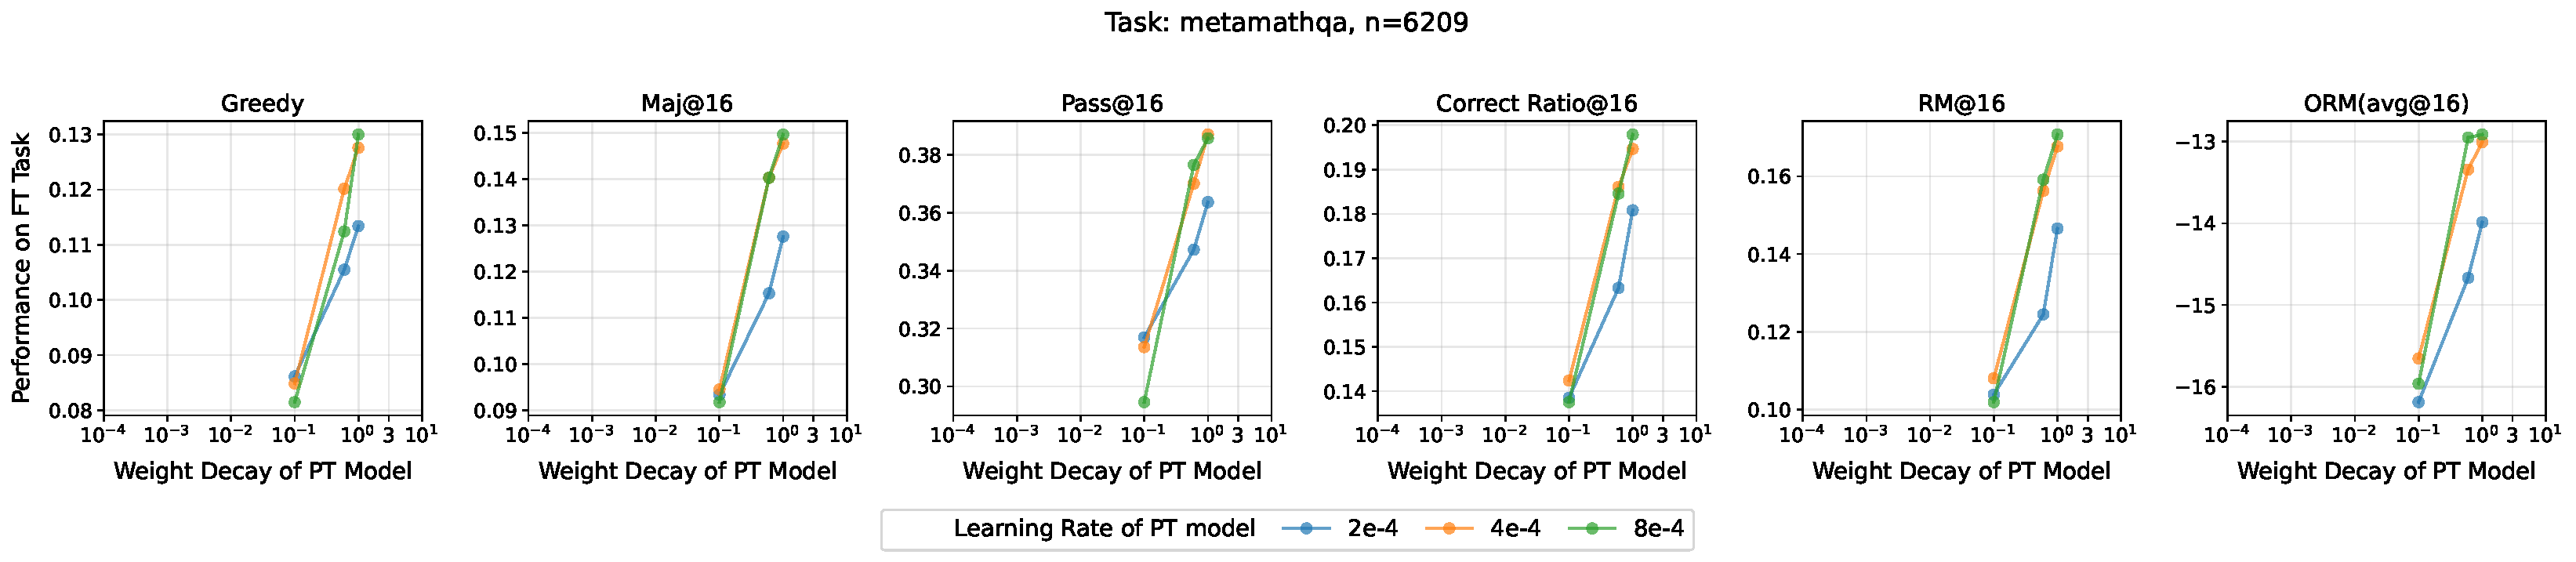
\includegraphics[width=\linewidth, trim={0 13mm 0 15mm}, clip]{figs/a08_vary_lr_during_pt/fixed_lr_vary_wd_metamathqa.pdf}
    \caption{\metamathqa{}{}}
    \end{subfigure}
    \begin{subfigure}[b]{0.88\textwidth} 
        \centering
        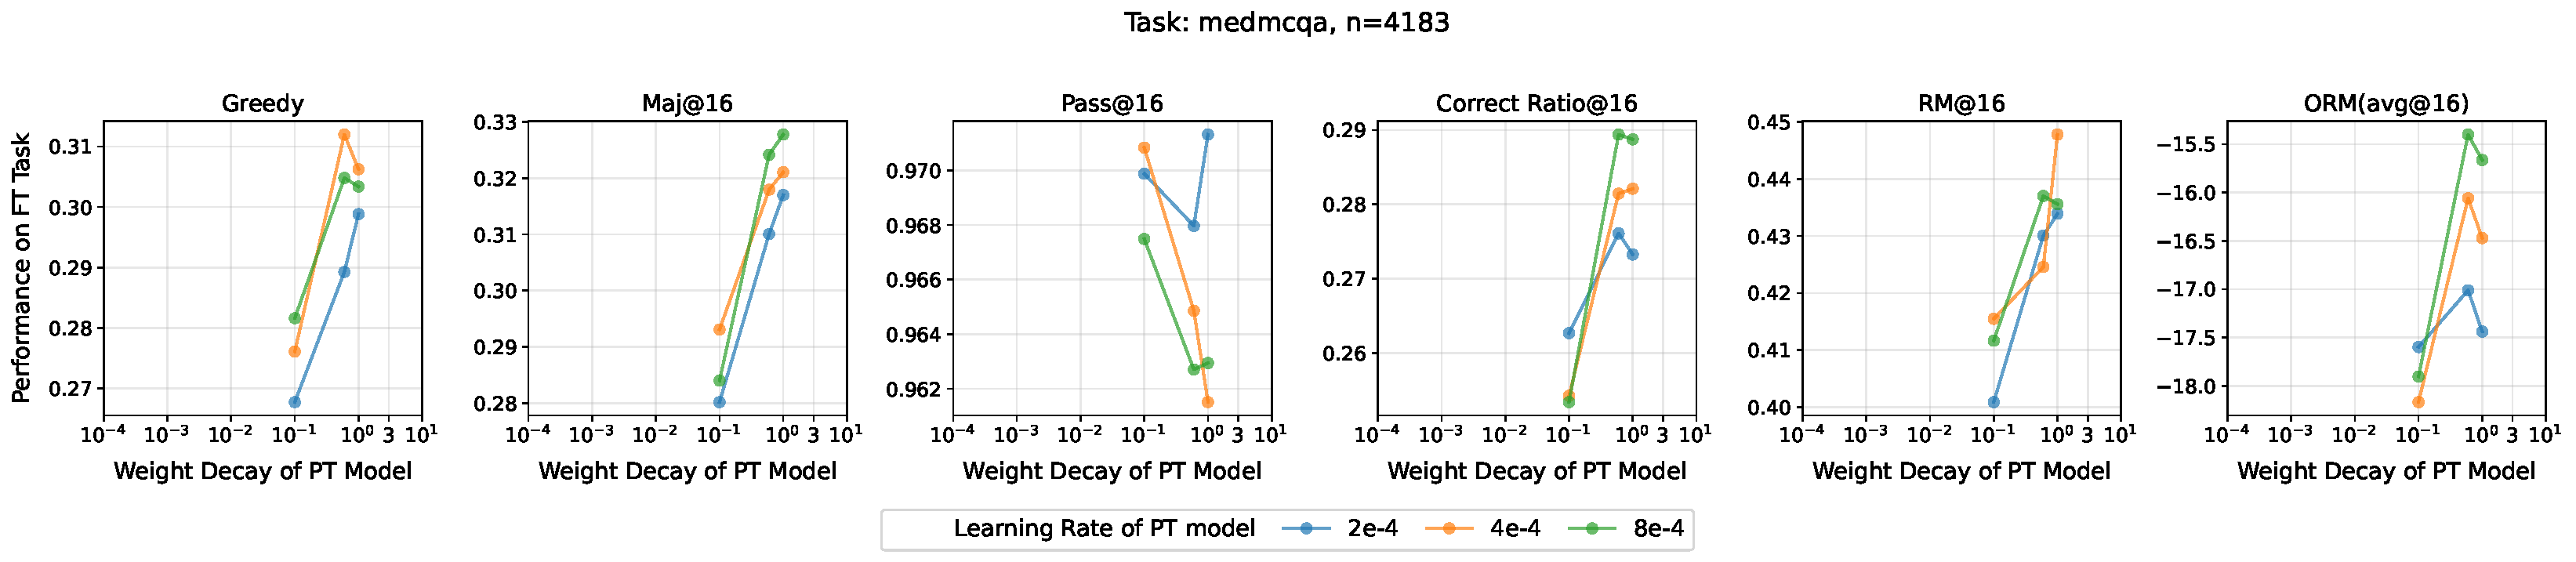
\includegraphics[width=\linewidth, trim={0 13mm 0 15mm}, clip]{figs/a08_vary_lr_during_pt/fixed_lr_vary_wd_medmcqa.pdf}
    \caption{\medmcqa{}{}}
    \end{subfigure}
    \begin{subfigure}[b]{0.88\textwidth} 
        \centering
        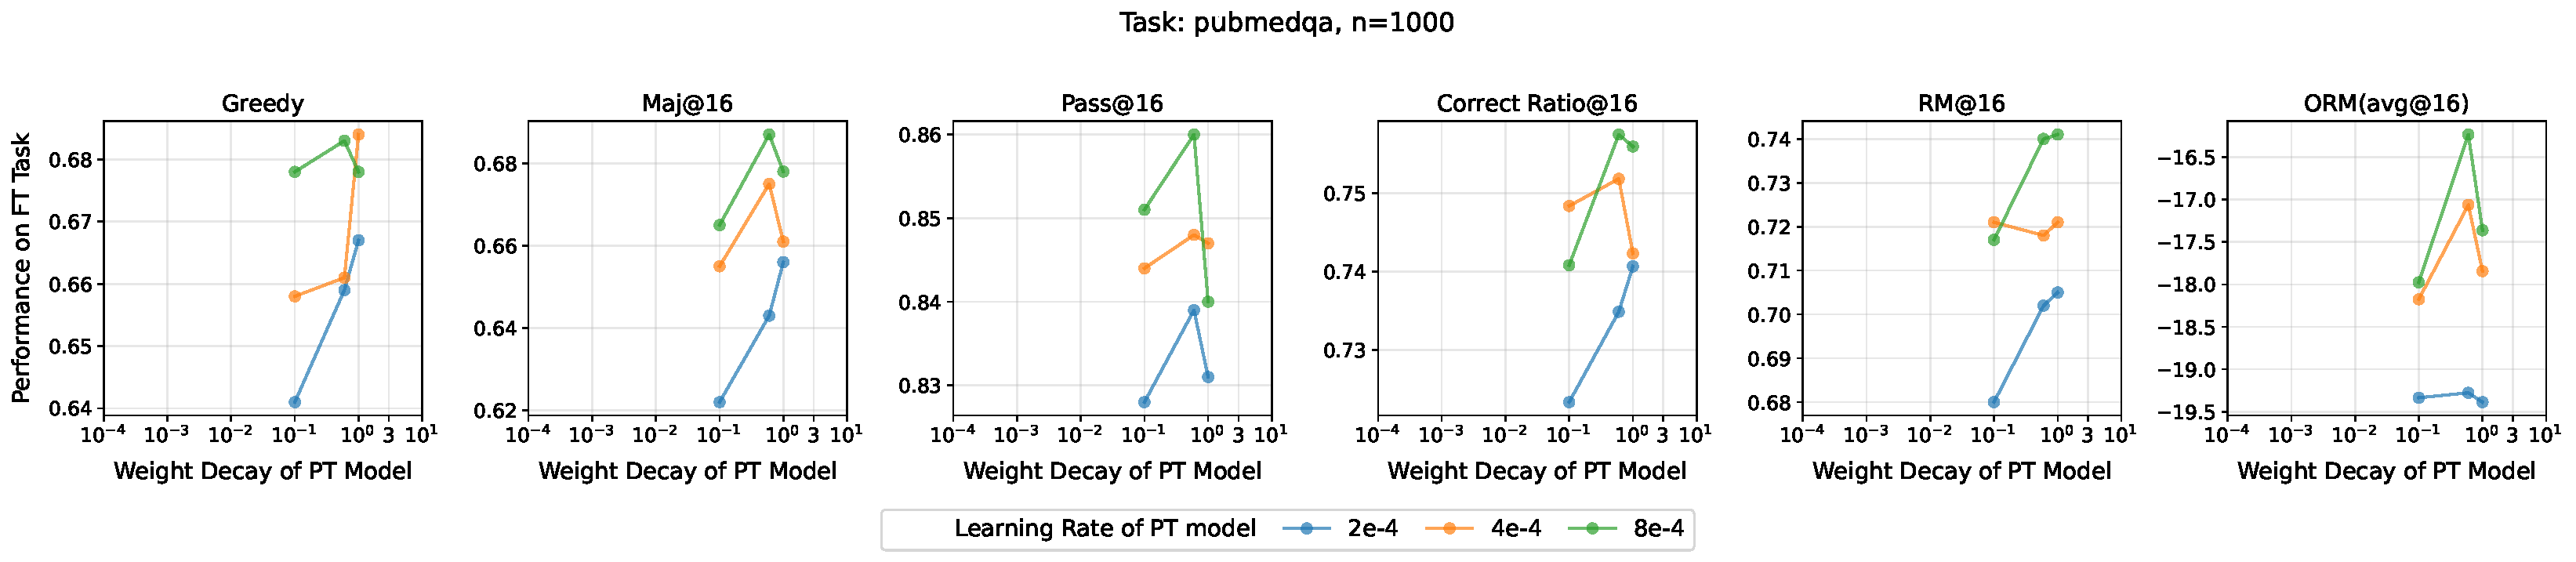
\includegraphics[width=\linewidth, trim={0 13mm 0 15mm}, clip]{figs/a08_vary_lr_during_pt/fixed_lr_vary_wd_pubmedqa.pdf}
    \caption{\pubmedqa{}{}}
    \end{subfigure}
    \begin{subfigure}[b]{0.88\textwidth} 
        \centering
        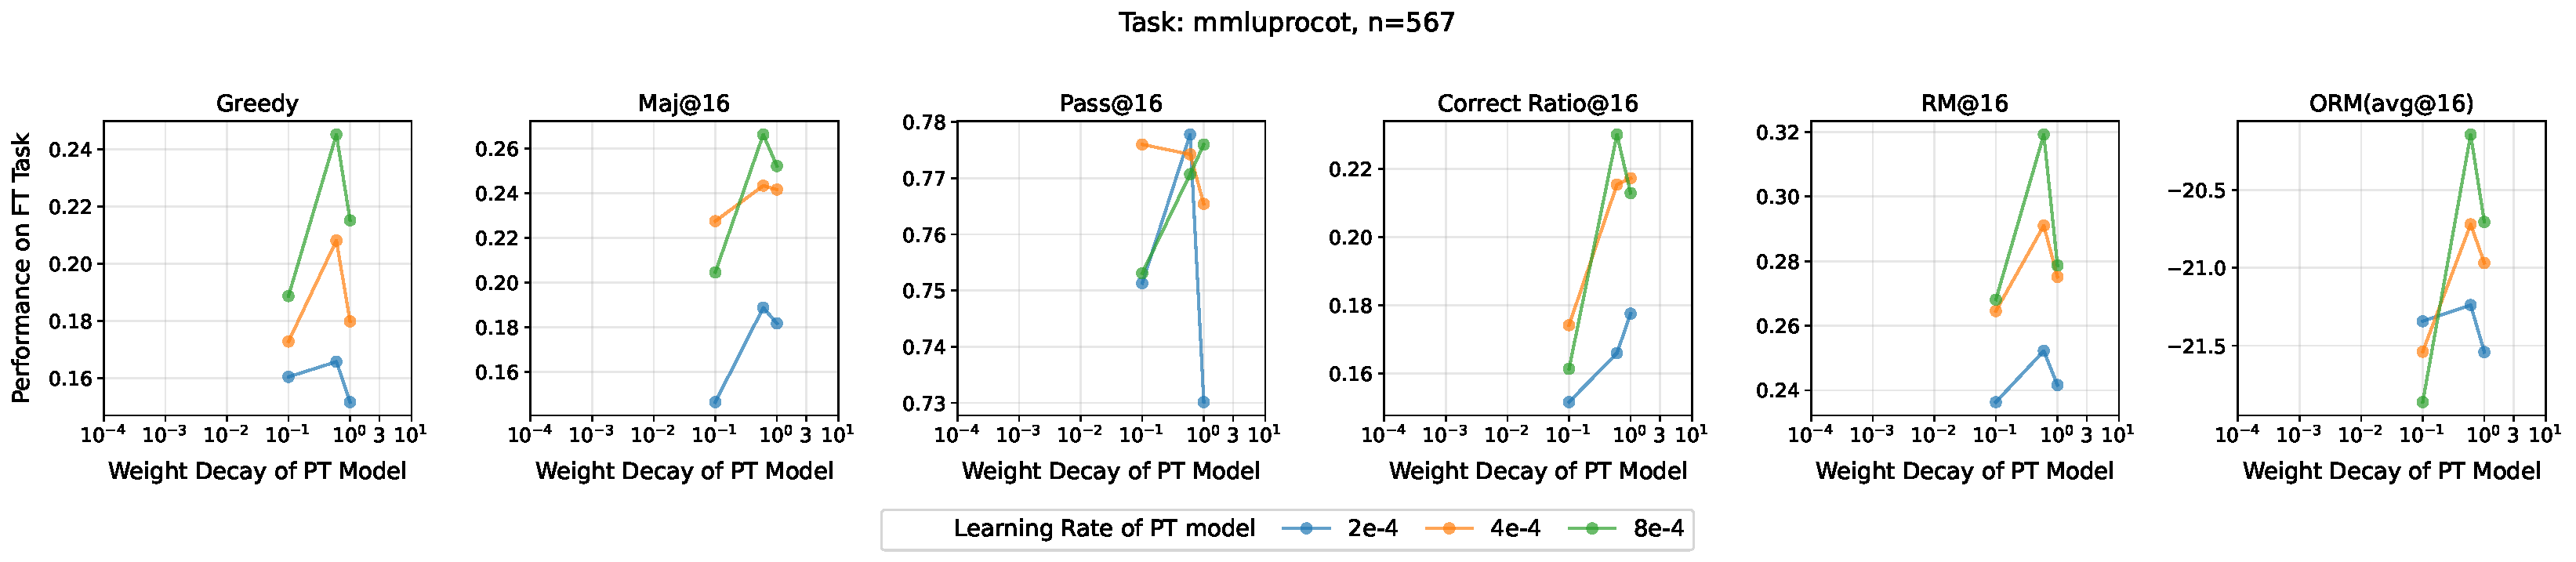
\includegraphics[width=\linewidth, trim={0 13mm 0 15mm}, clip]{figs/a08_vary_lr_during_pt/fixed_lr_vary_wd_mmluprocot.pdf}
    \caption{\mmluprocot{}{}}
    \end{subfigure}
    \begin{subfigure}[b]{0.88\textwidth} 
        \centering
        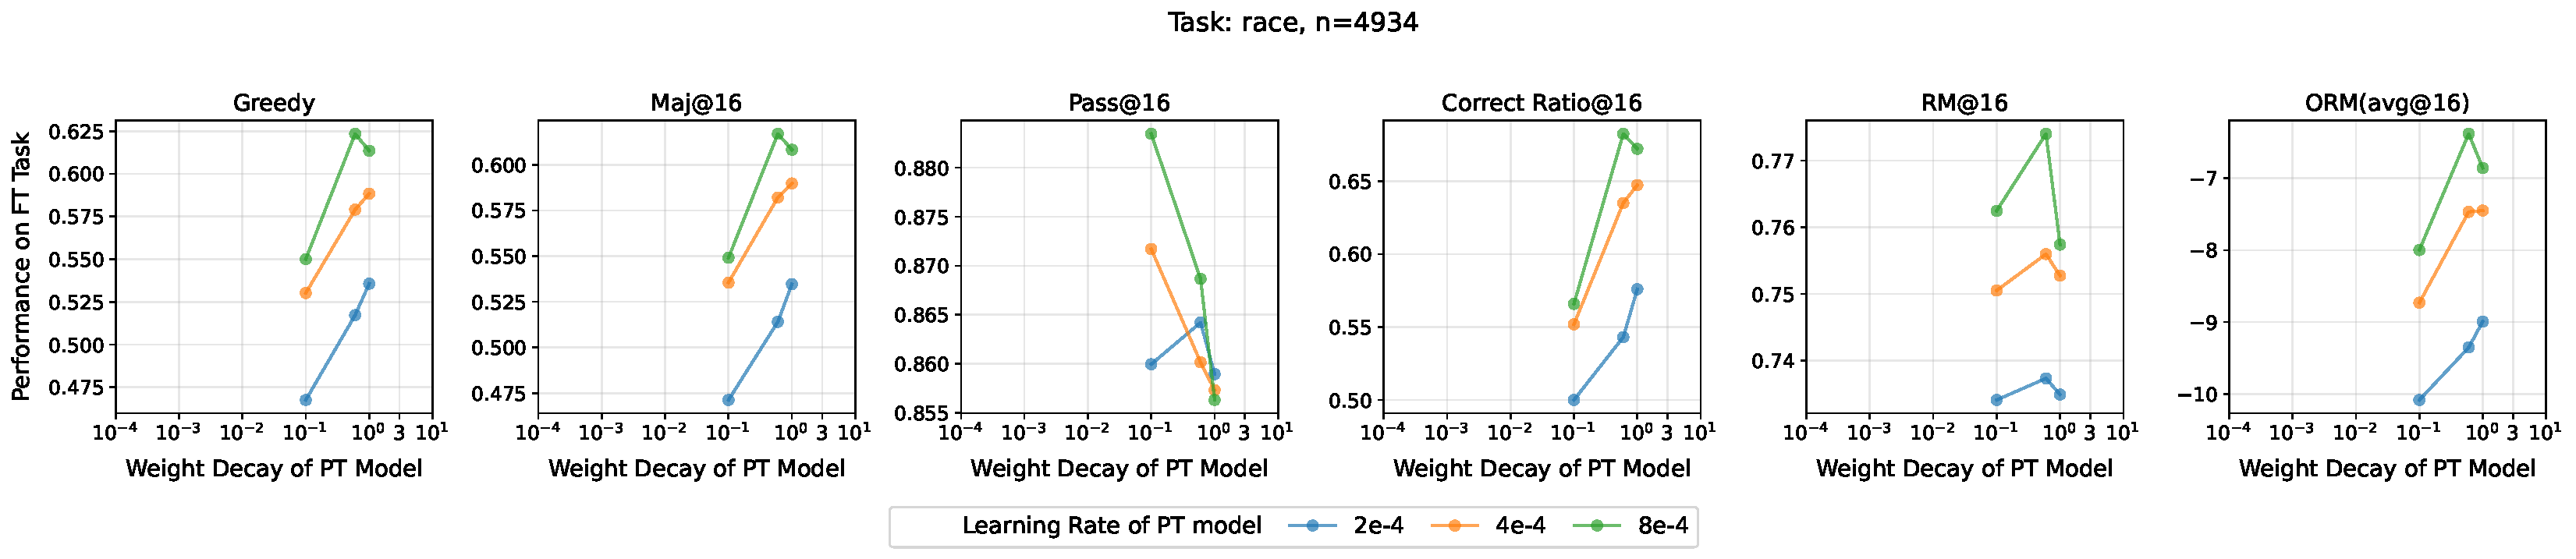
\includegraphics[width=\linewidth, trim={0 13mm 0 15mm}, clip]{figs/a08_vary_lr_during_pt/fixed_lr_vary_wd_race.pdf}
    \caption{\race{}}
    \end{subfigure}
    \begin{subfigure}[b]{0.88\textwidth} 
        \centering
        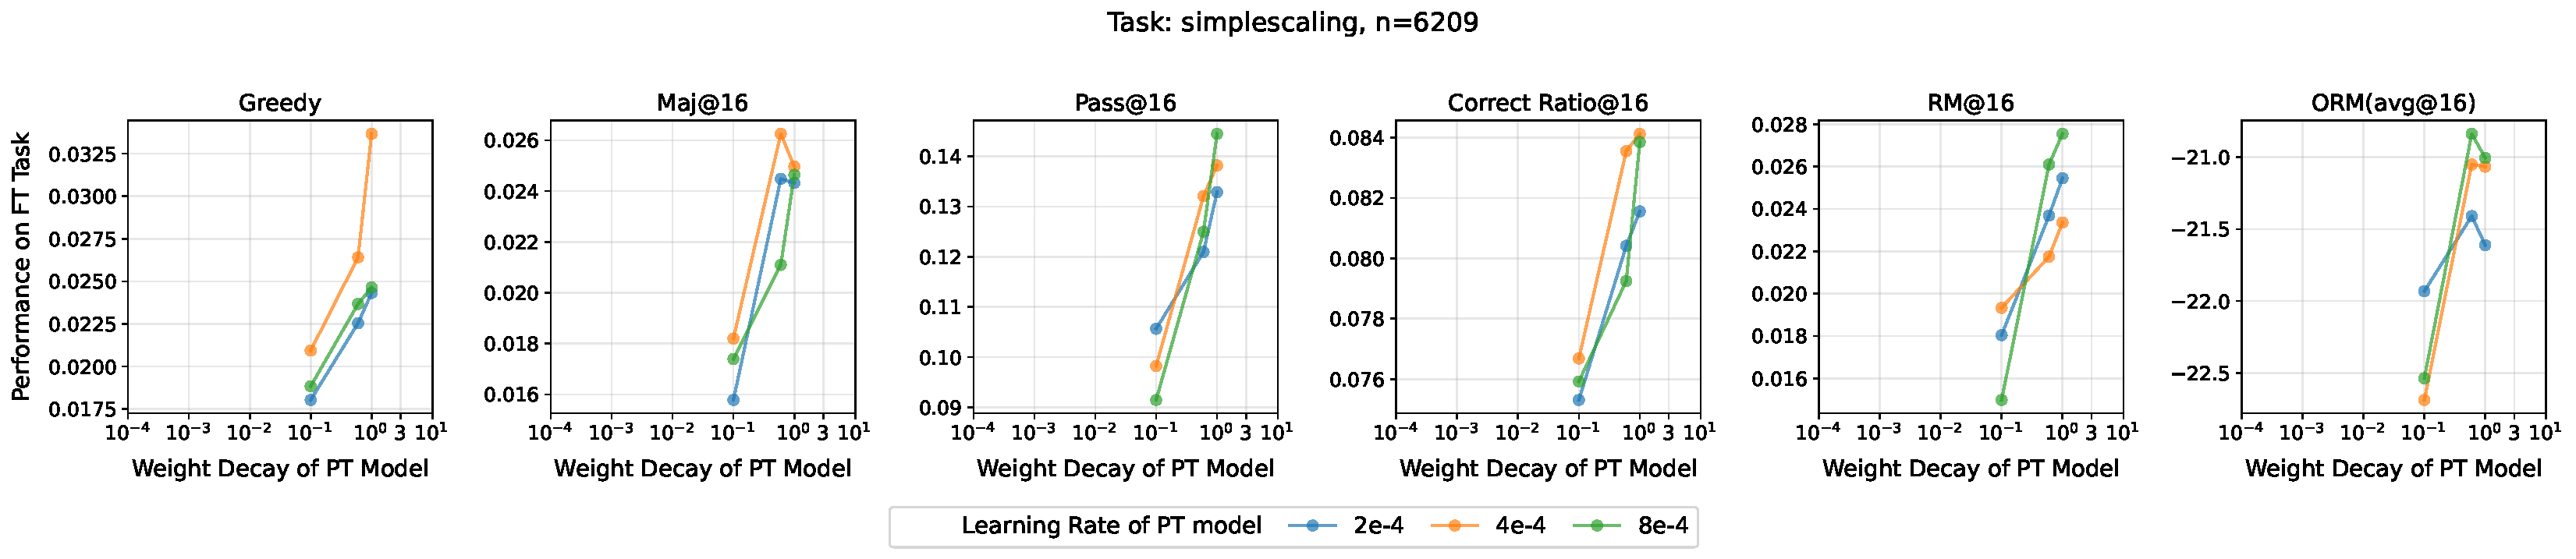
\includegraphics[width=\linewidth, trim={0 13mm 0 15mm}, clip]{figs/a08_vary_lr_during_pt/fixed_lr_vary_wd_simplescaling.pdf}
    \caption{\simplescaling{}}
    \end{subfigure}
    \begin{subfigure}[b]{0.88\textwidth} 
        \centering
        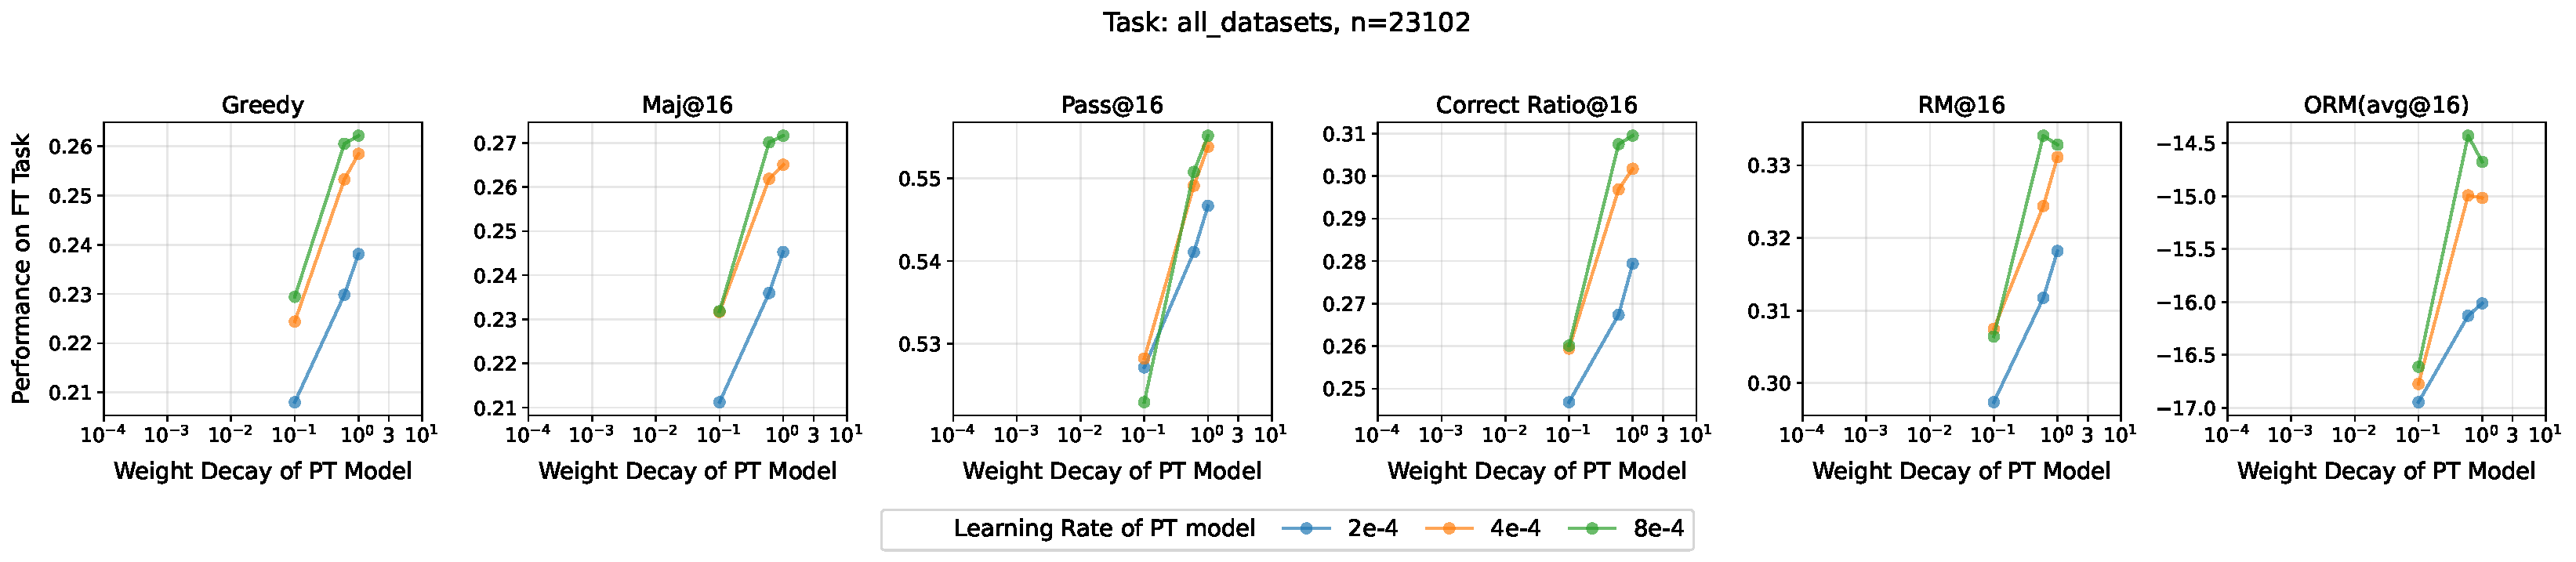
\includegraphics[width=\linewidth, trim={0 0 0 15mm}, clip]{figs/a08_vary_lr_during_pt/fixed_lr_vary_wd_all_datasets.pdf}
    \caption{Average over datasets}
    \end{subfigure}
    \caption{{\bf Effect of pretraining hyperparameters on model plasticity.} Models are pretrained with varying weight decay and learning rates. Across learning rates, higher weight decay during pretraining leads to greater model plasticty and higher downstream performance.}
    \label{fig:app-hyperparam-exp-pt--fixed-lr-vary-wd}
\end{figure*}




\begin{figure*}[h] 
    \centering
    \begin{subfigure}[b]{0.88\textwidth} 
        \centering
        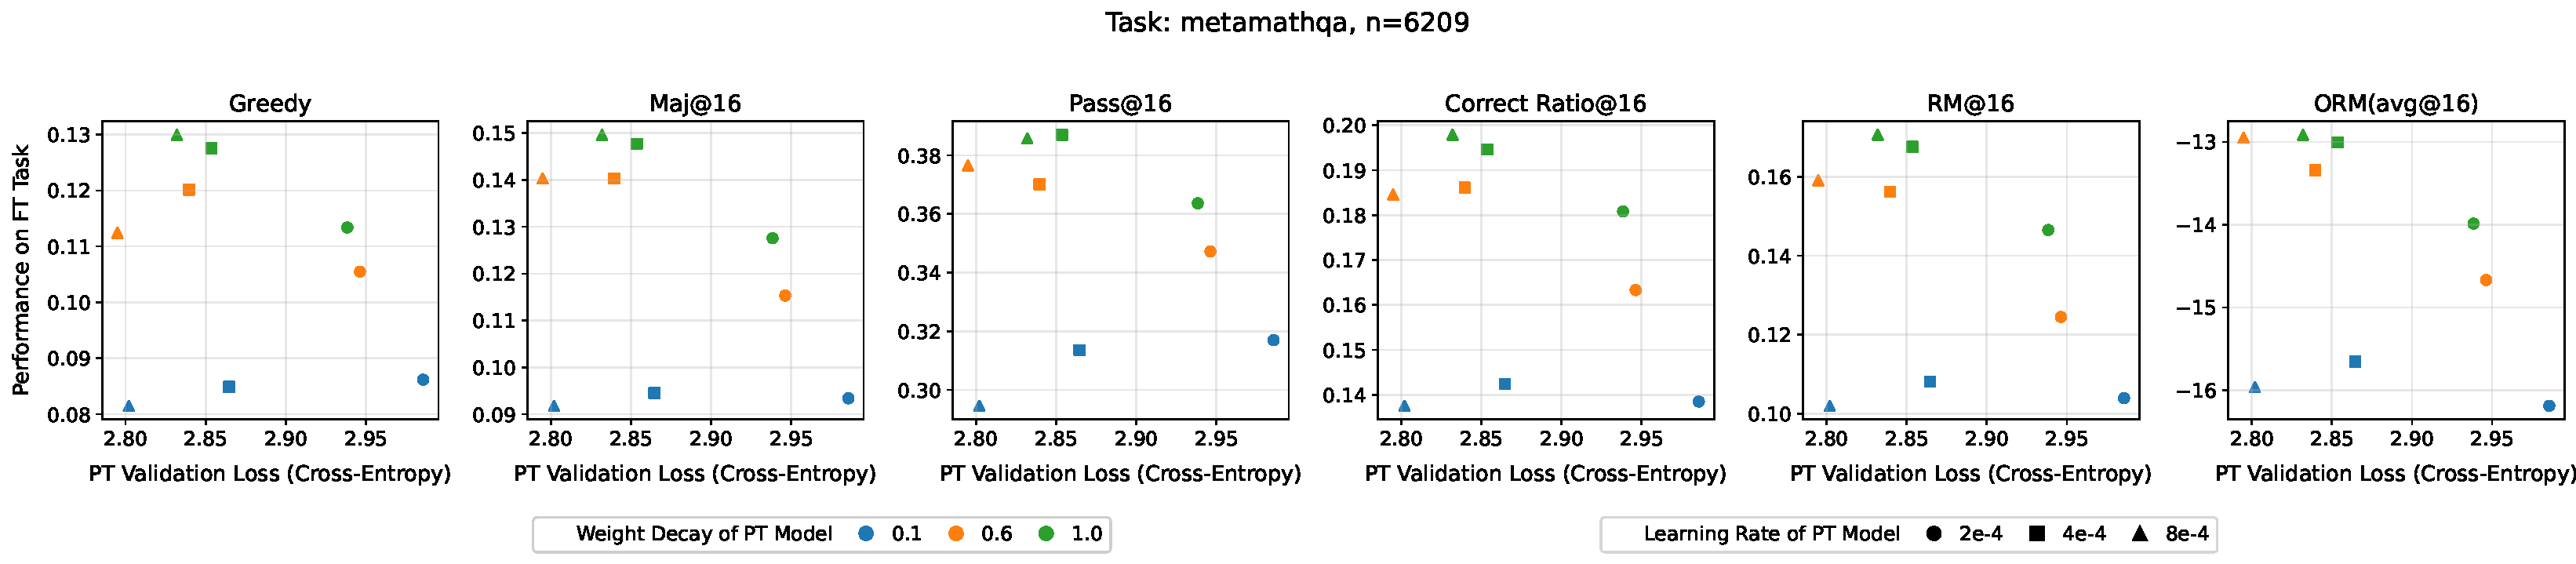
\includegraphics[width=\linewidth, trim={0 13mm 0 15mm}, clip]{figs/a08_vary_lr_during_pt/val_loss_vs_ft_acc_metamathqa.pdf}
    \caption{\metamathqa{}{}}
    \end{subfigure}
    \begin{subfigure}[b]{0.88\textwidth} 
        \centering
        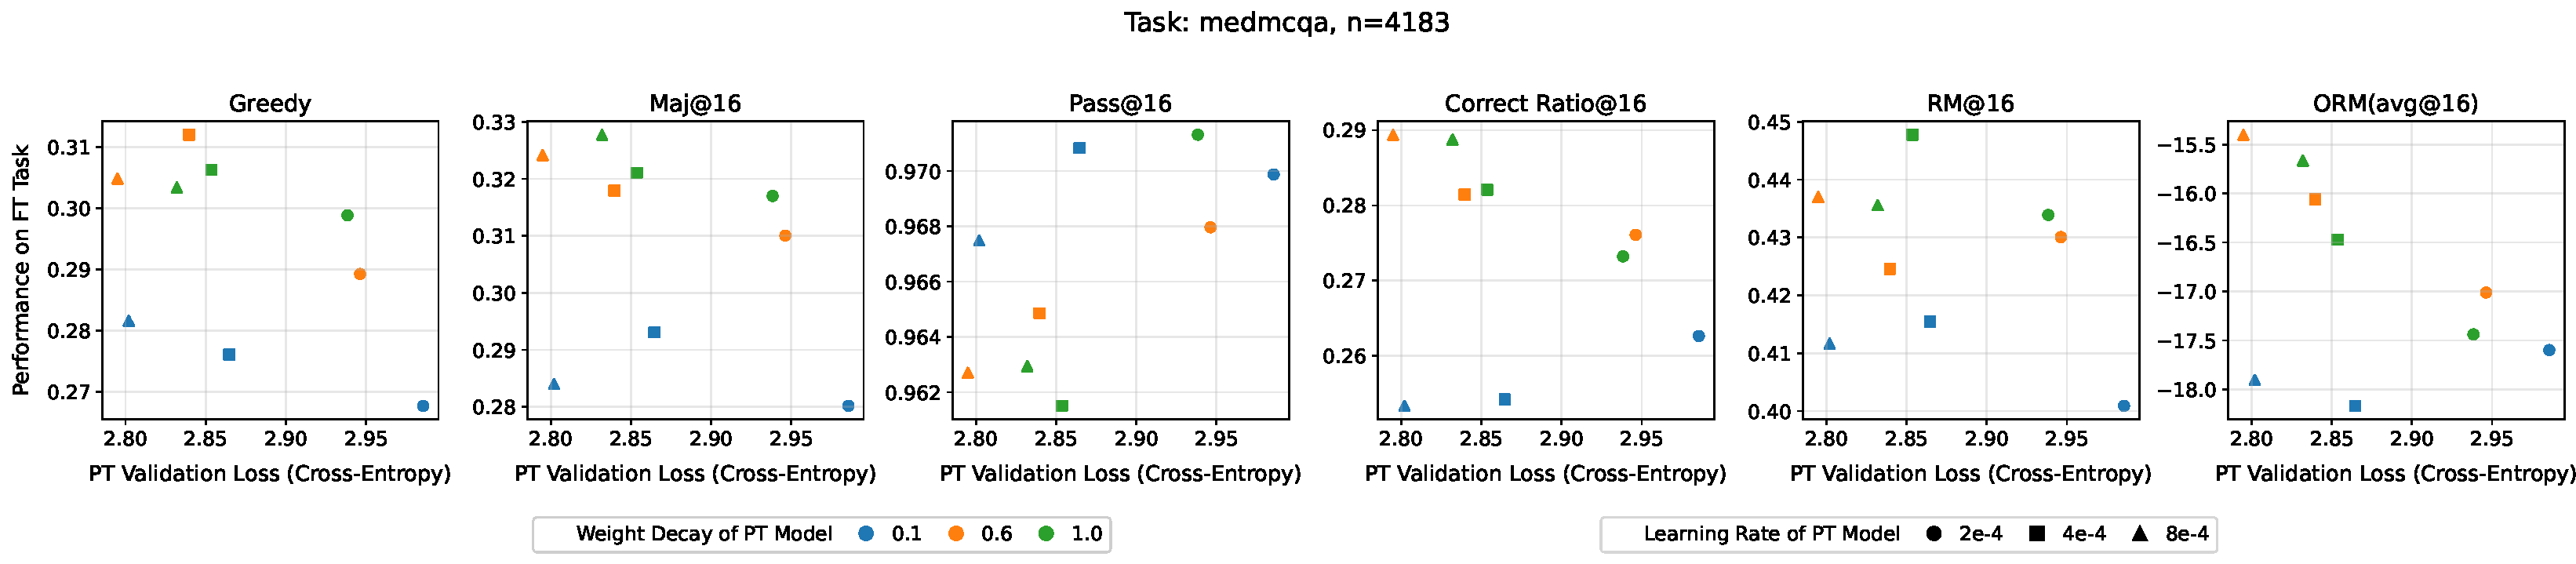
\includegraphics[width=\linewidth, trim={0 13mm 0 15mm}, clip]{figs/a08_vary_lr_during_pt/val_loss_vs_ft_acc_medmcqa.pdf}
    \caption{\medmcqa{}{}}
    \end{subfigure}
    \begin{subfigure}[b]{0.88\textwidth} 
        \centering
        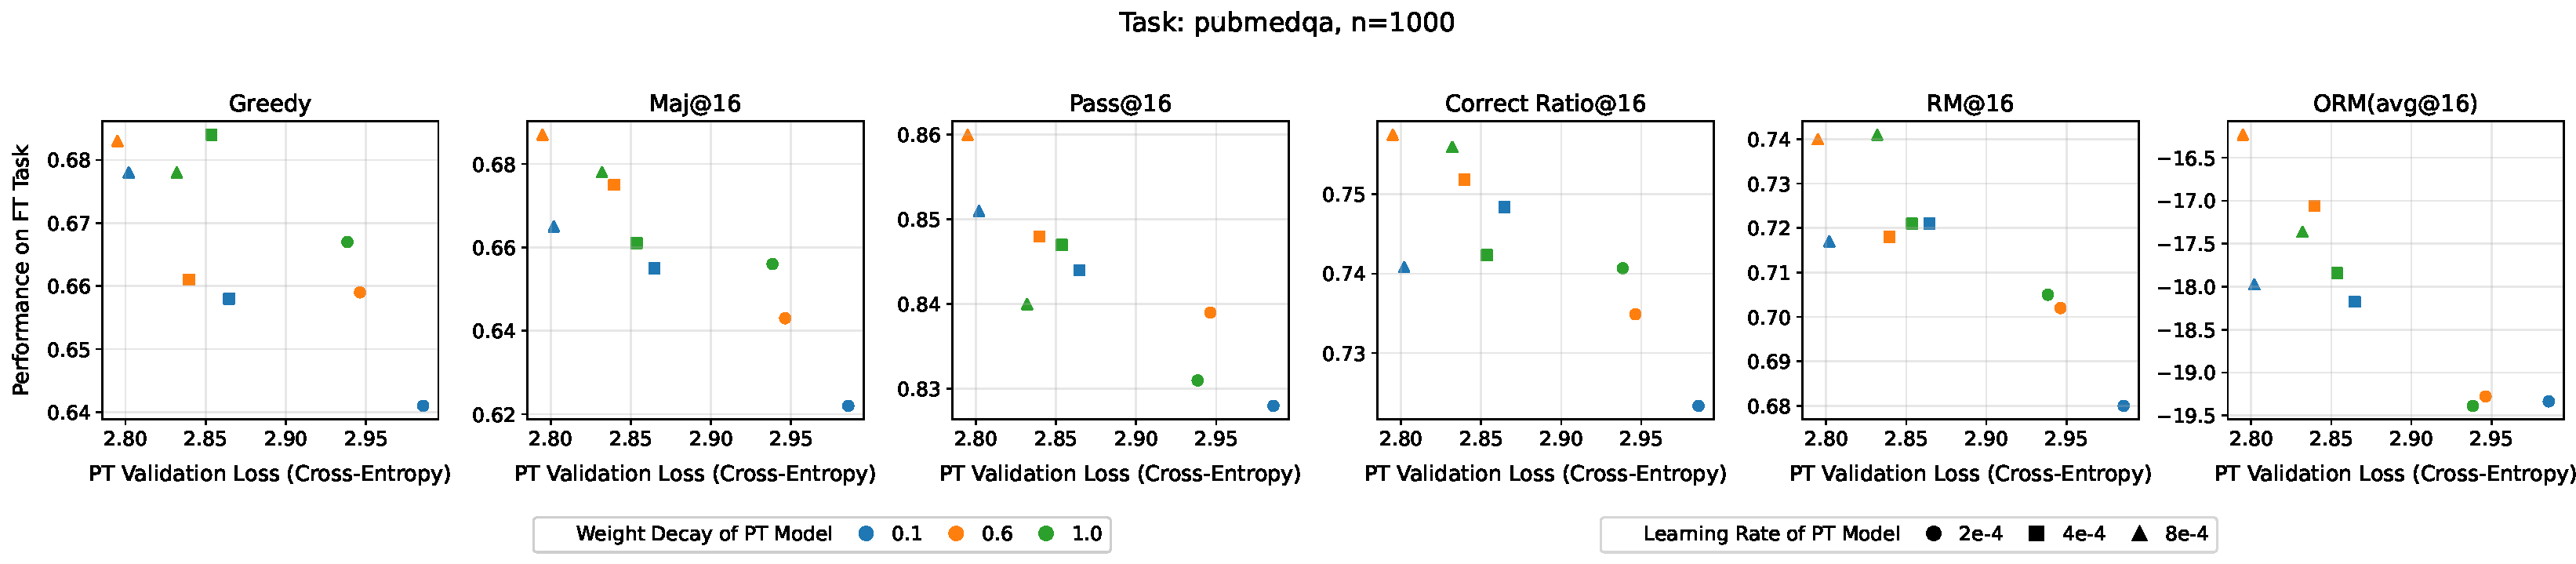
\includegraphics[width=\linewidth, trim={0 13mm 0 15mm}, clip]{figs/a08_vary_lr_during_pt/val_loss_vs_ft_acc_pubmedqa.pdf}
    \caption{\pubmedqa{}{}}
    \end{subfigure}
    \begin{subfigure}[b]{0.88\textwidth} 
        \centering
        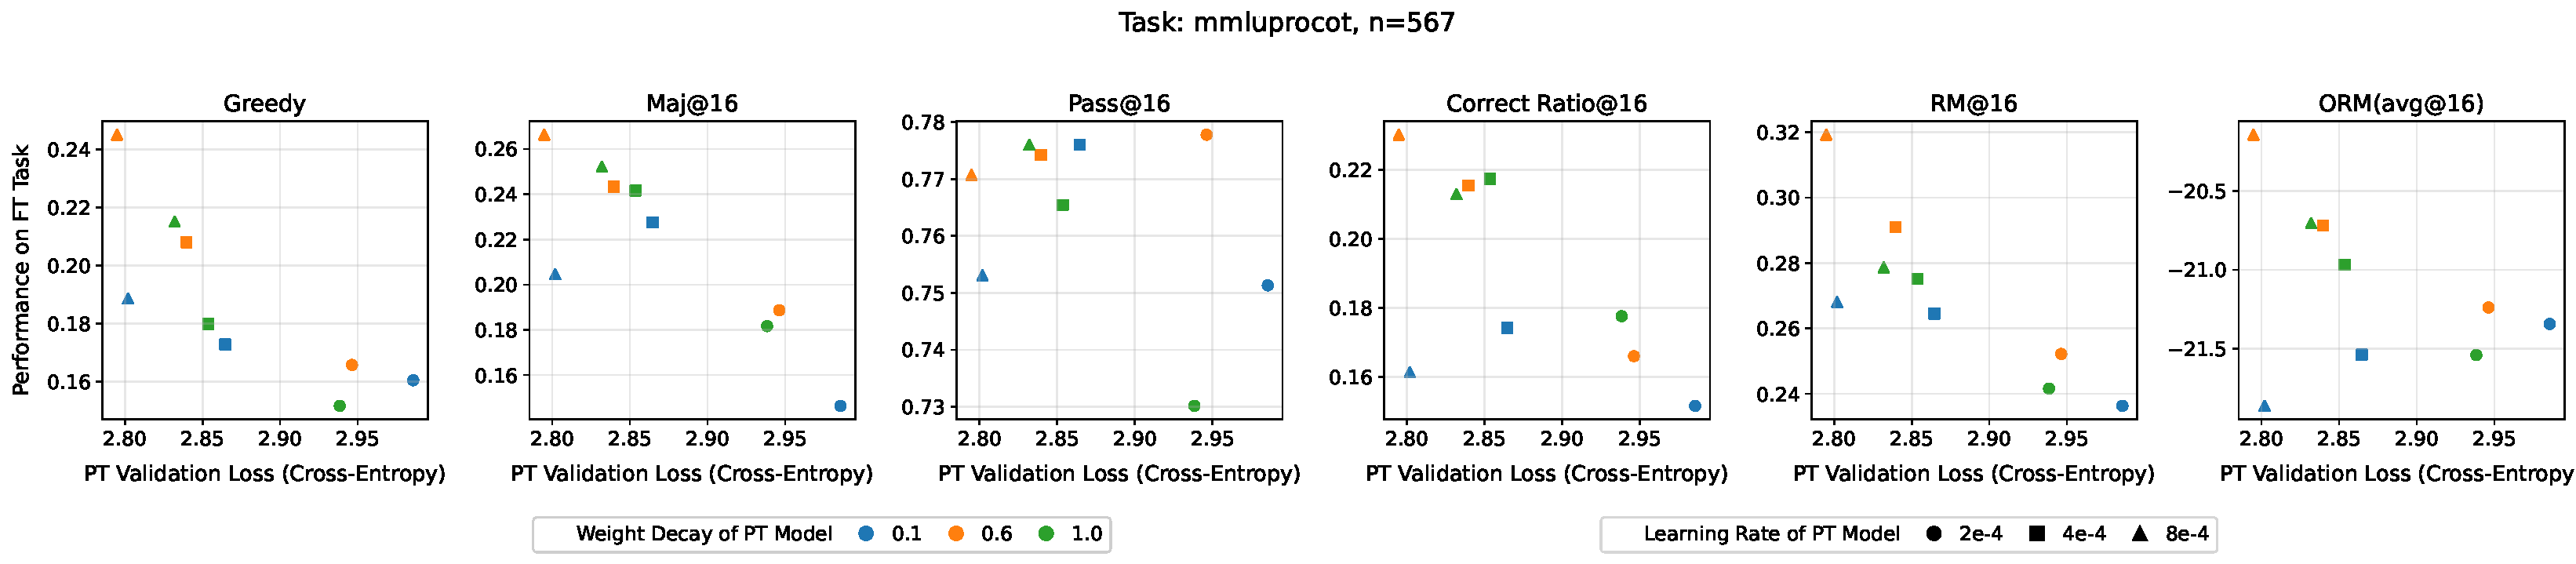
\includegraphics[width=\linewidth, trim={0 13mm 0 15mm}, clip]{figs/a08_vary_lr_during_pt/val_loss_vs_ft_acc_mmluprocot.pdf}
    \caption{\mmluprocot{}{}}
    \end{subfigure}
    \begin{subfigure}[b]{0.88\textwidth} 
        \centering
        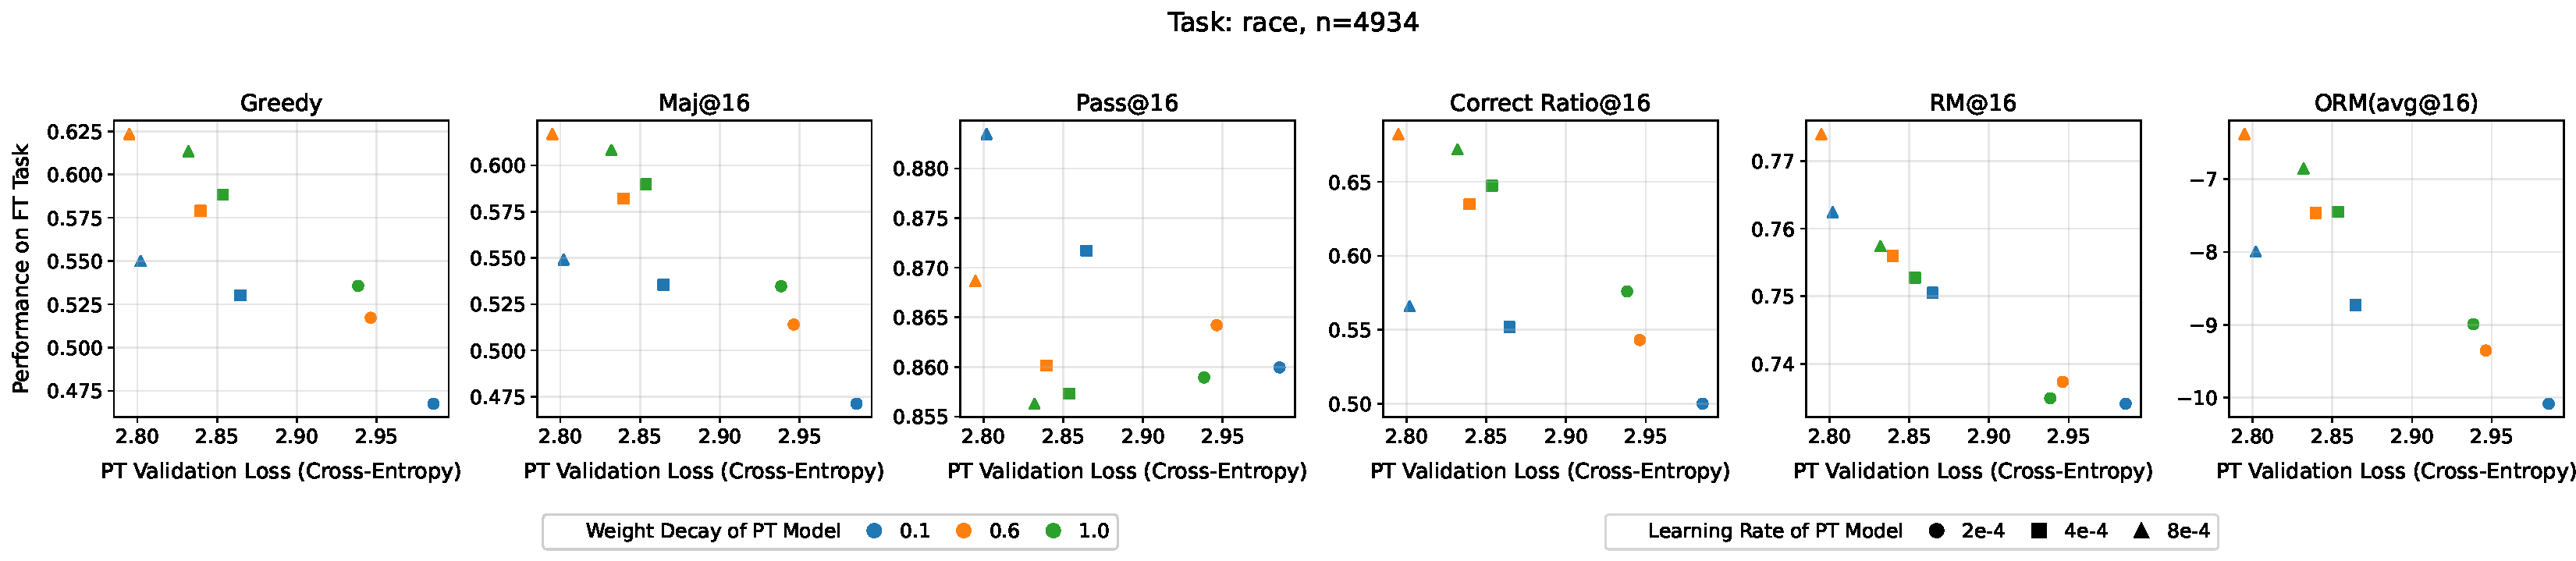
\includegraphics[width=\linewidth, trim={0 13mm 0 15mm}, clip]{figs/a08_vary_lr_during_pt/val_loss_vs_ft_acc_race.pdf}
    \caption{\race{}}
    \end{subfigure}
    \begin{subfigure}[b]{0.88\textwidth} 
        \centering
        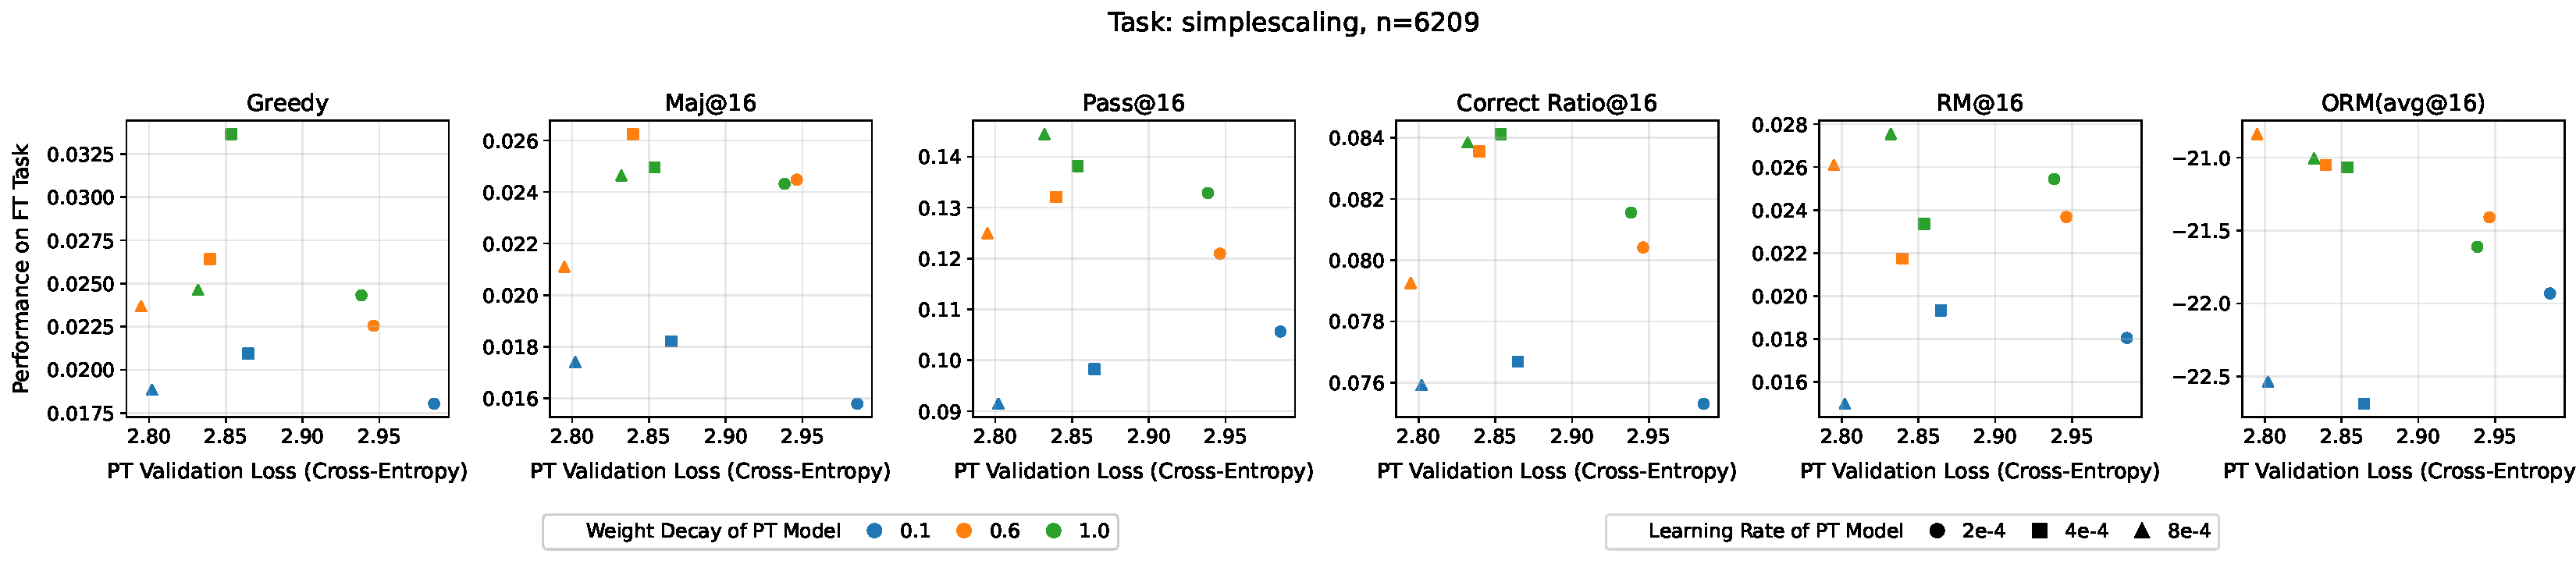
\includegraphics[width=\linewidth, trim={0 13mm 0 15mm}, clip]{figs/a08_vary_lr_during_pt/val_loss_vs_ft_acc_simplescaling.pdf}
    \caption{\simplescaling{}}
    \end{subfigure}
    \begin{subfigure}[b]{0.88\textwidth} 
        \centering
        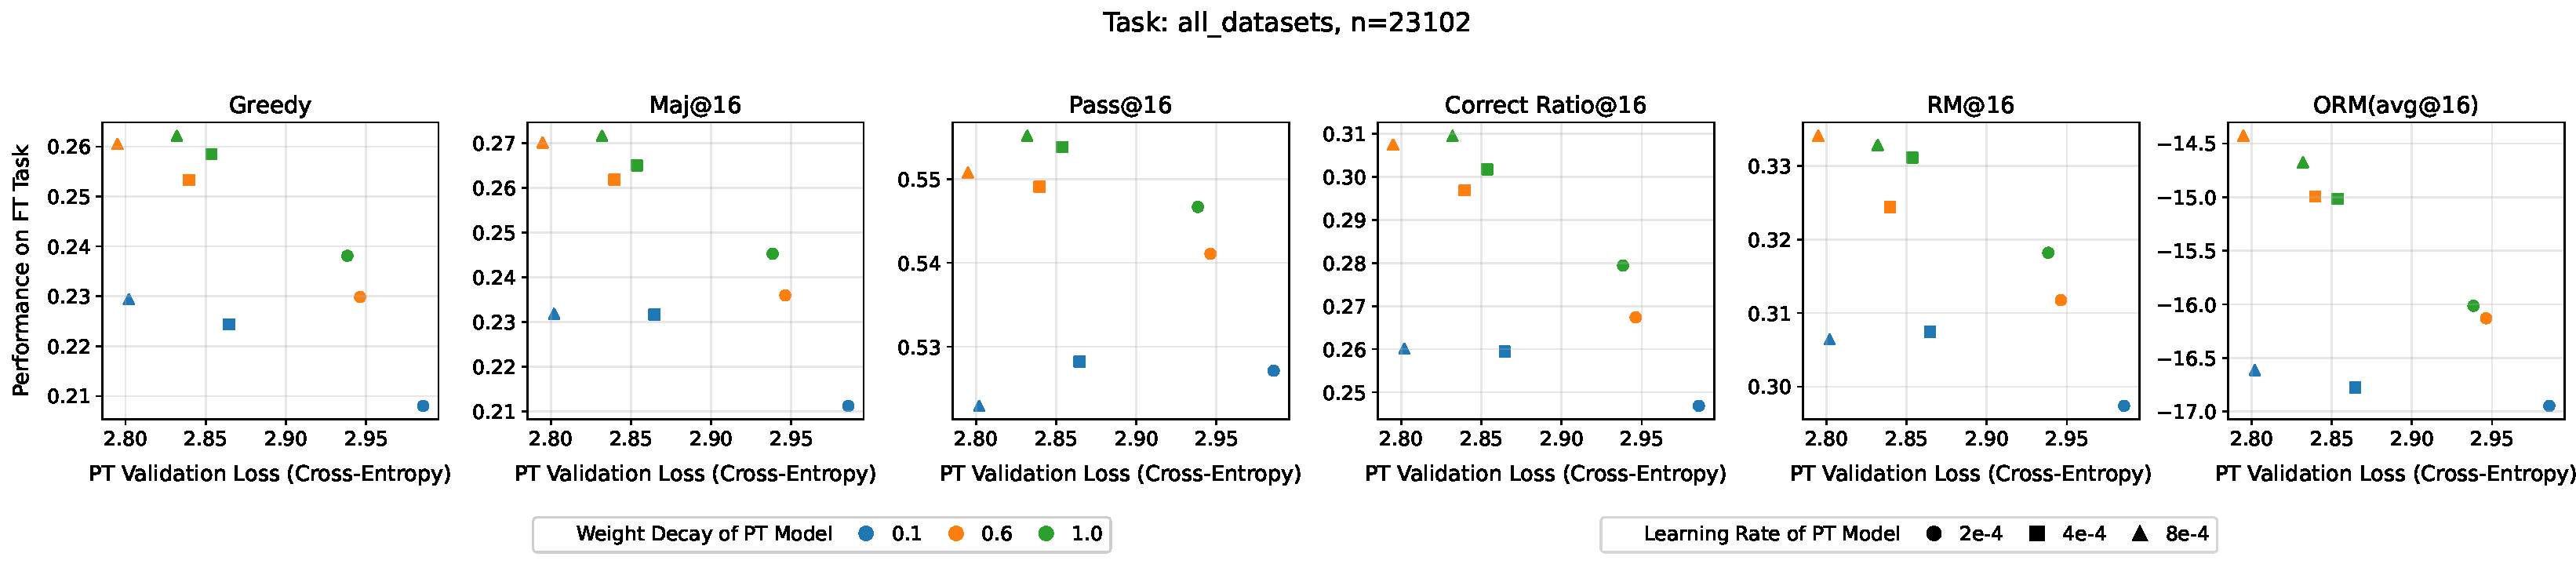
\includegraphics[width=\linewidth, trim={0 0 0 15mm}, clip]{figs/a08_vary_lr_during_pt/val_loss_vs_ft_acc_all_datasets.pdf}
    \caption{Average over datasets}
    \end{subfigure}
    \caption{{\bf Pretraining (PT) performance is not perfectly predictive of fine-tuning (FT) performance.} 
    Fixing learning rate, the weight decay that leads to the best PT loss does not always lead to the best FT loss. Overall, the model with best PT loss is not the model with best FT loss.}
    \label{fig:app-hyperparam-exp-pt--pt-vs-ft-perf}
\end{figure*}




\begin{figure*}[h] 
    \centering

    \begin{subfigure}[b]{\textwidth}
        \centering
        \makebox[\textwidth][c]{
            \hspace{-4mm}
            \raisebox{7.5mm}{\makebox[18mm][r]{\shortstack[l]{lr = 1e-5\\bs = 32}}}
            \hspace{2mm}
            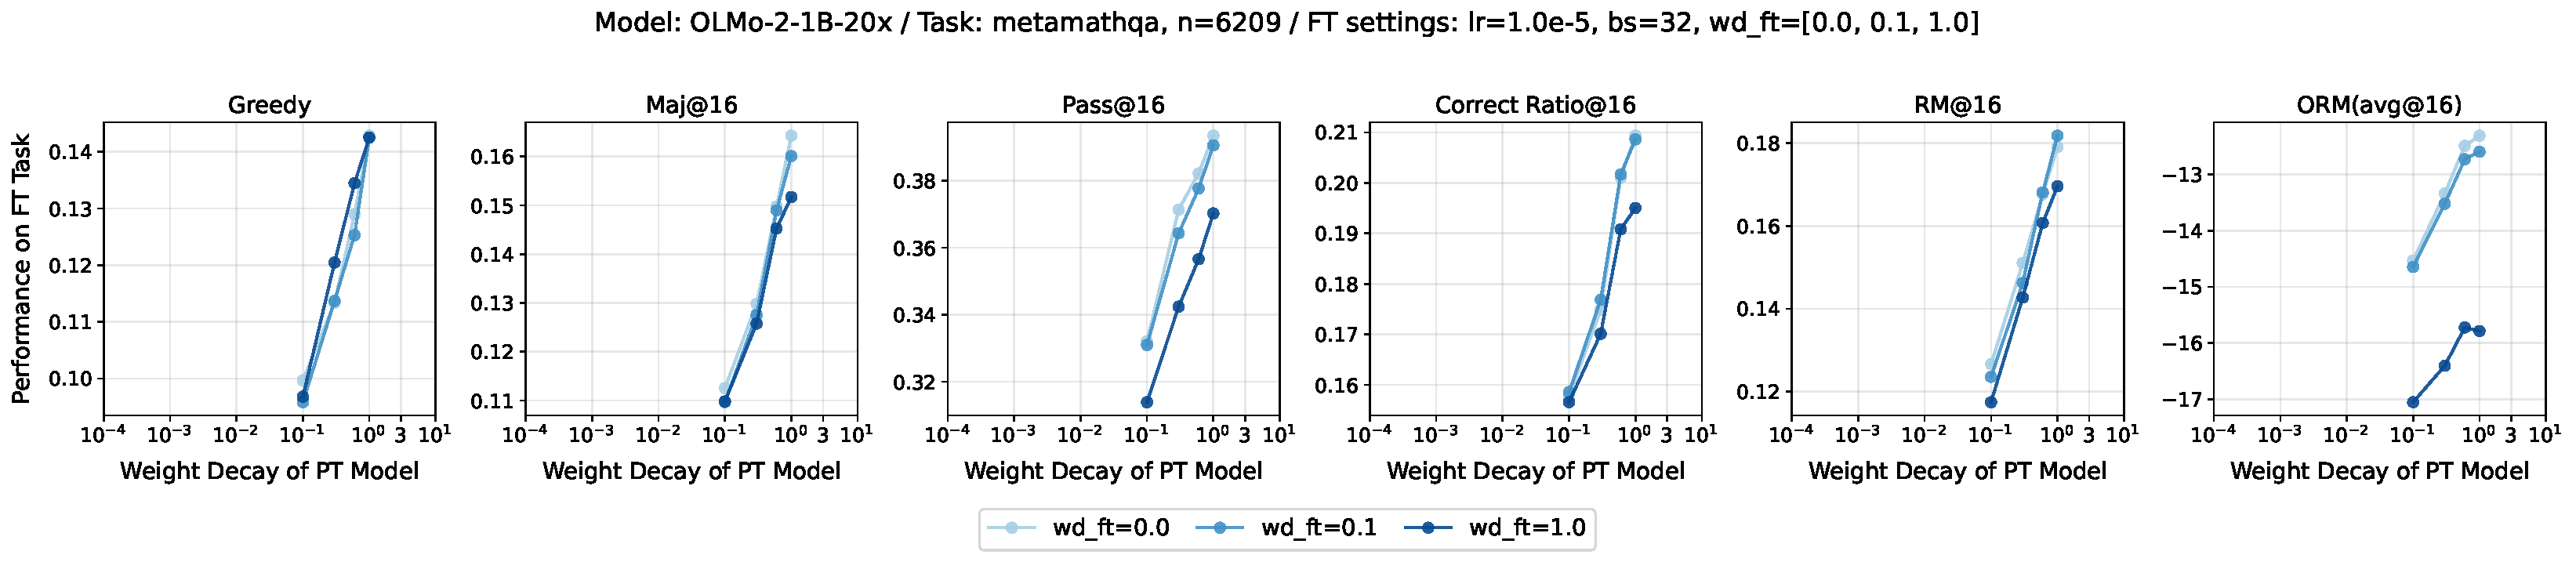
\includegraphics[width=0.92\textwidth, trim={0 25mm 0 20mm}, clip]{figs/a06_ft_sweep/ft_sweep_olmo-1B-30BT_metamathqa_lr1.0e-5_bs32.pdf}%
        }
    \end{subfigure}

    \begin{subfigure}[b]{\textwidth}
        \centering
        \makebox[\textwidth][c]{
            \hspace{-4mm}
            \raisebox{7.5mm}{\makebox[18mm][r]{\shortstack[l]{lr = 1e-5\\bs = 64}}}
            \hspace{2mm}
            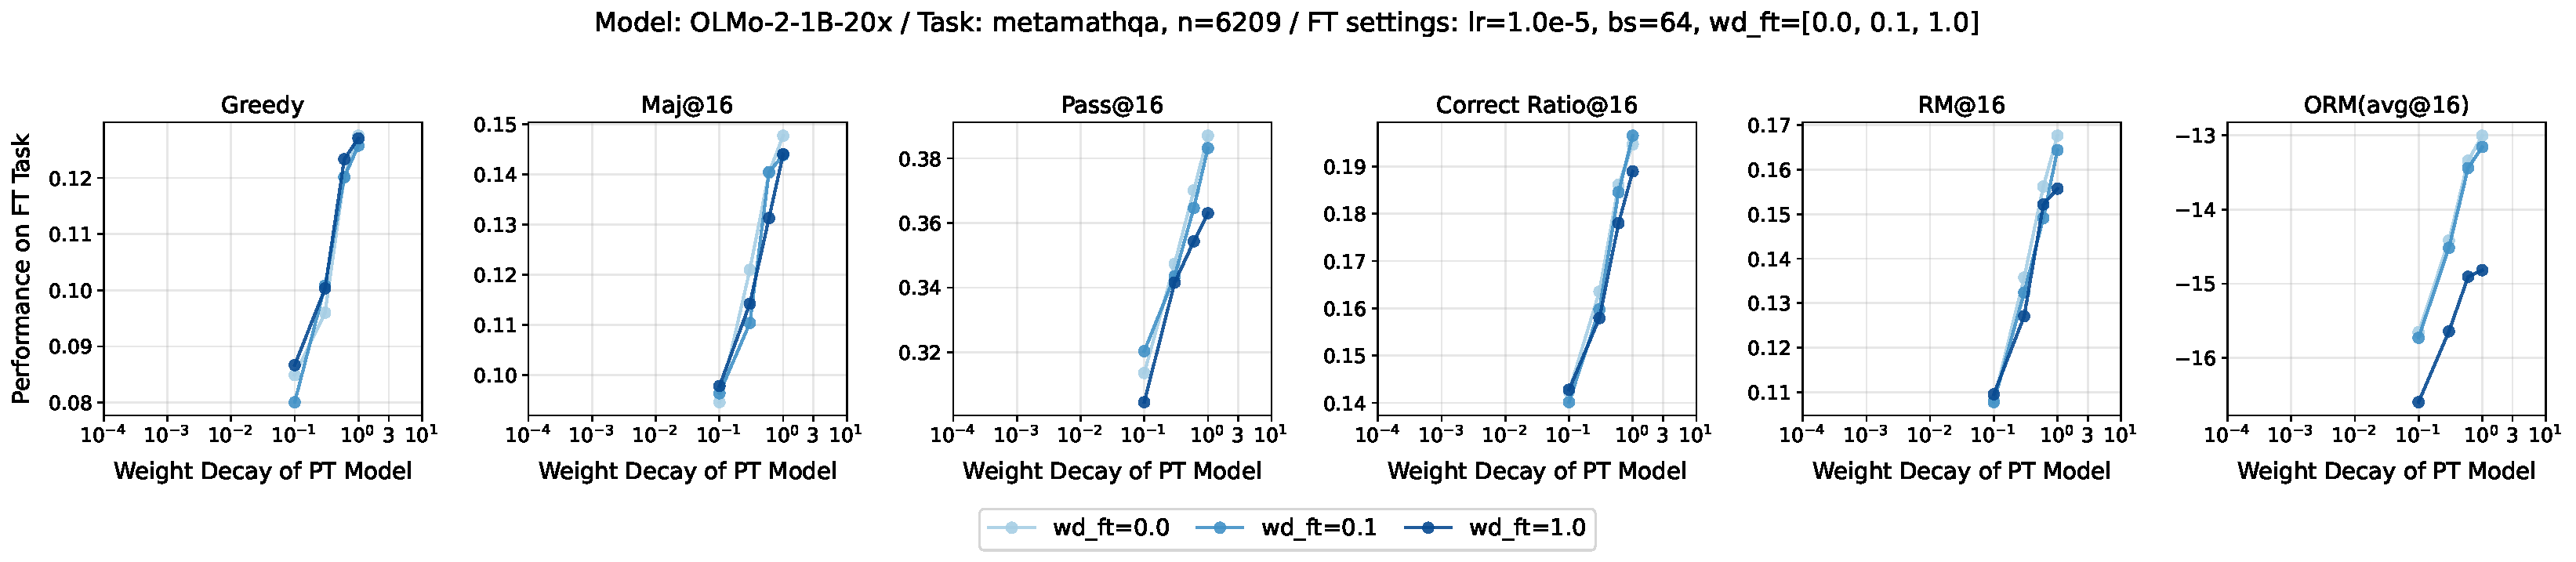
\includegraphics[width=0.92\textwidth, trim={0 25mm 0 25mm}, clip]{figs/a06_ft_sweep/ft_sweep_olmo-1B-30BT_metamathqa_lr1.0e-5_bs64.pdf}%
        }
    \end{subfigure}

    \begin{subfigure}[b]{\textwidth}
        \centering
        \makebox[\textwidth][c]{
            \hspace{-4mm}
            \raisebox{7.5mm}{\makebox[18mm][r]{\shortstack[l]{lr = 1e-5\\bs = 128}}}
            \hspace{2mm}
            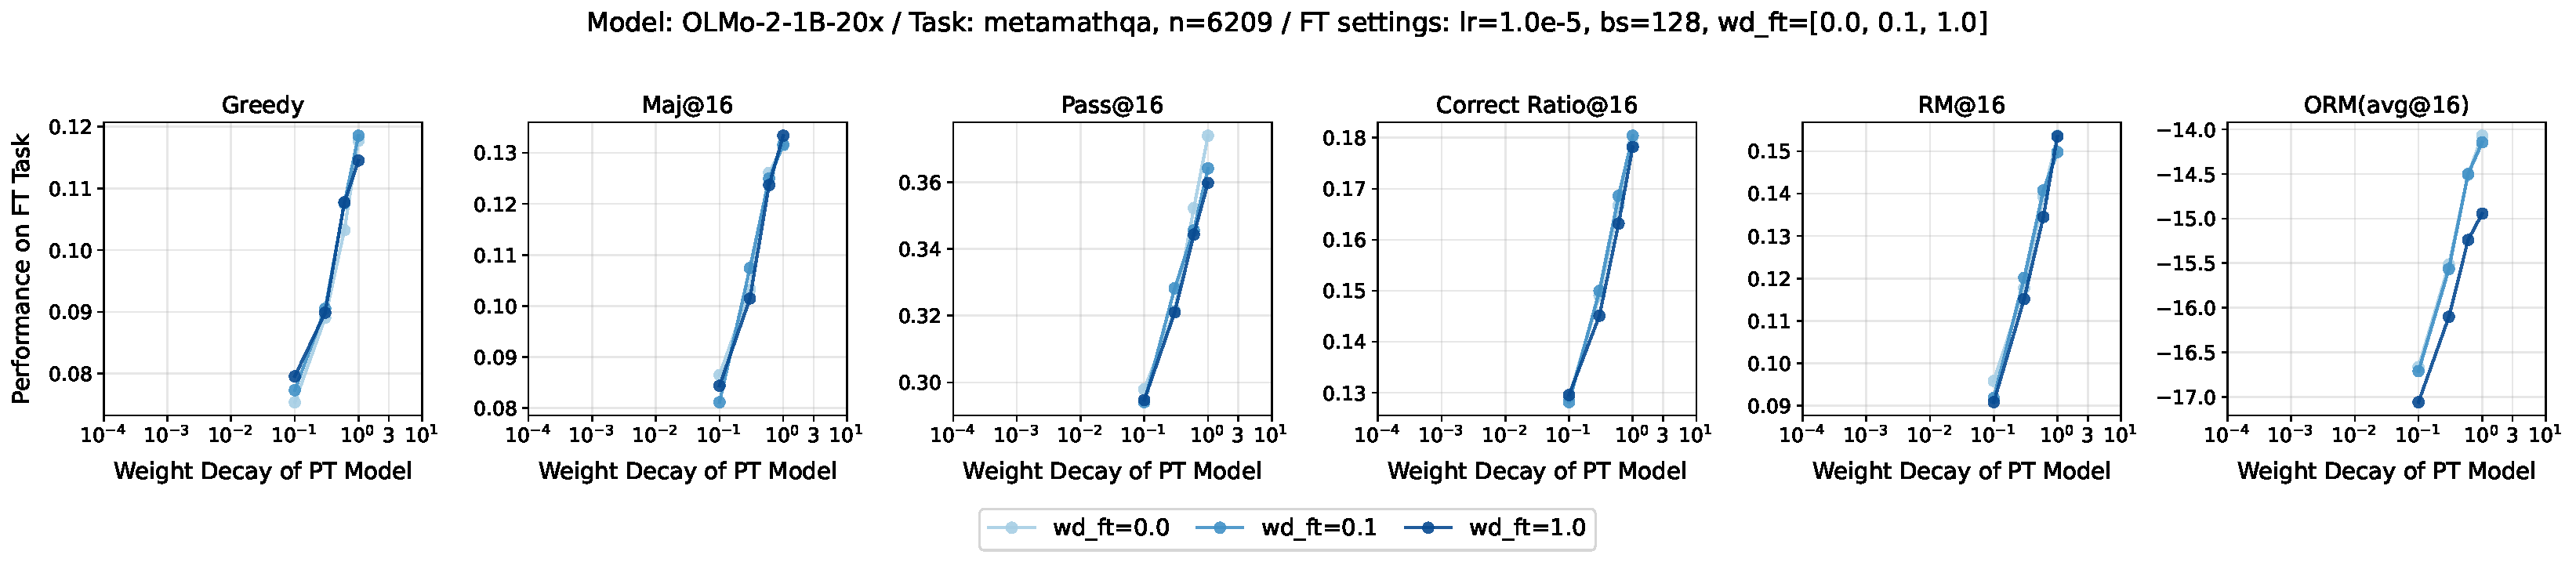
\includegraphics[width=0.92\textwidth, trim={0 25mm 0 25mm}, clip]{figs/a06_ft_sweep/ft_sweep_olmo-1B-30BT_metamathqa_lr1.0e-5_bs128.pdf}%
        }
    \end{subfigure}

    \begin{subfigure}[b]{\textwidth}
        \centering
        \makebox[\textwidth][c]{
            \hspace{-4mm}
            \raisebox{7.5mm}{\makebox[18mm][r]{\shortstack[l]{lr = 3e-5\\bs = 32}}}
            \hspace{2mm}
            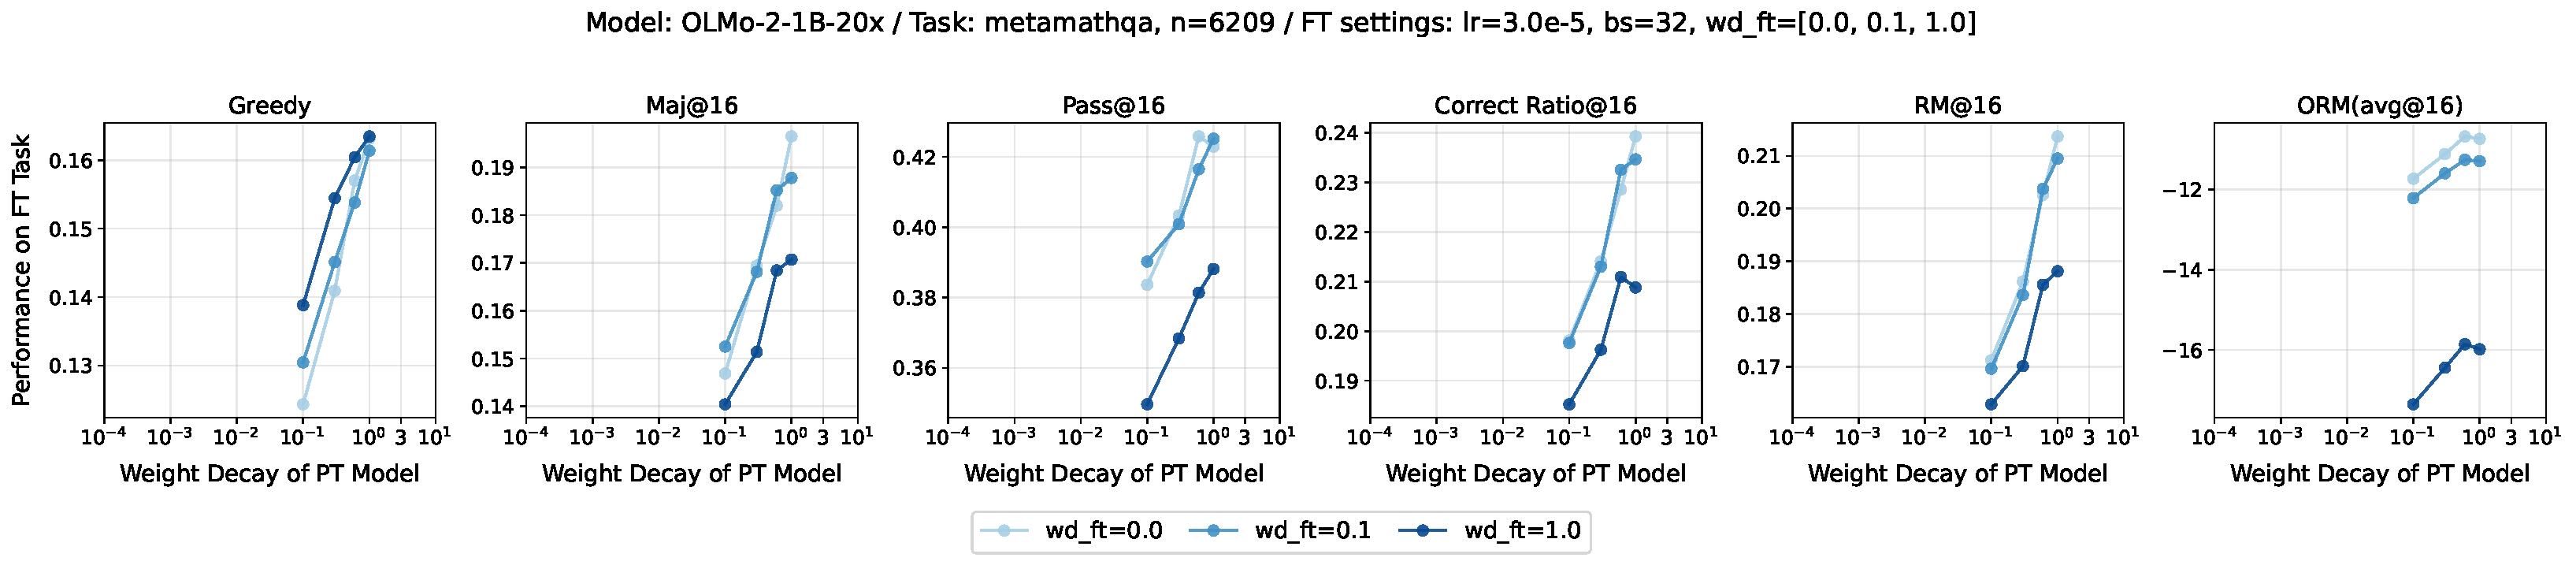
\includegraphics[width=0.92\textwidth, trim={0 25mm 0 25mm}, clip]{figs/a06_ft_sweep/ft_sweep_olmo-1B-30BT_metamathqa_lr3.0e-5_bs32.pdf}%
        }
    \end{subfigure}

    \begin{subfigure}[b]{\textwidth}
        \centering
        \makebox[\textwidth][c]{
            \hspace{-4mm}
            \raisebox{7.5mm}{\makebox[18mm][r]{\shortstack[l]{lr = 3e-5\\bs = 64}}}
            \hspace{2mm}
            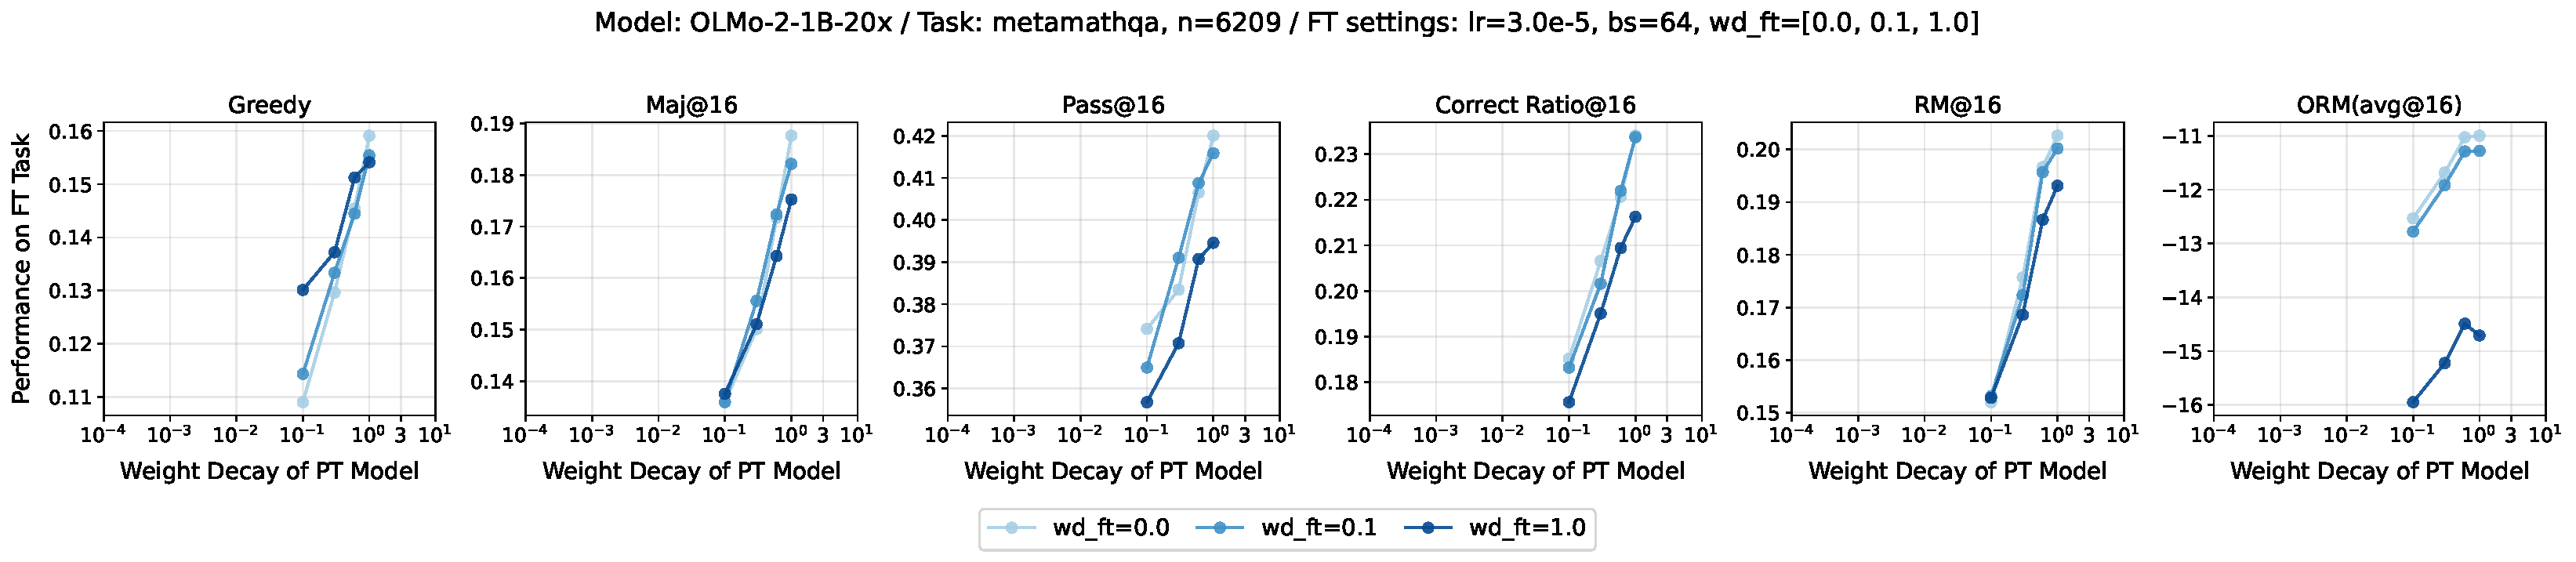
\includegraphics[width=0.92\textwidth, trim={0 25mm 0 25mm}, clip]{figs/a06_ft_sweep/ft_sweep_olmo-1B-30BT_metamathqa_lr3.0e-5_bs64.pdf}%
        }
    \end{subfigure}

    \begin{subfigure}[b]{\textwidth}
        \centering
        \makebox[\textwidth][c]{
            \hspace{-4mm}
            \raisebox{7.5mm}{\makebox[18mm][r]{\shortstack[l]{lr = 3e-5\\bs = 128}}}
            \hspace{2mm}
            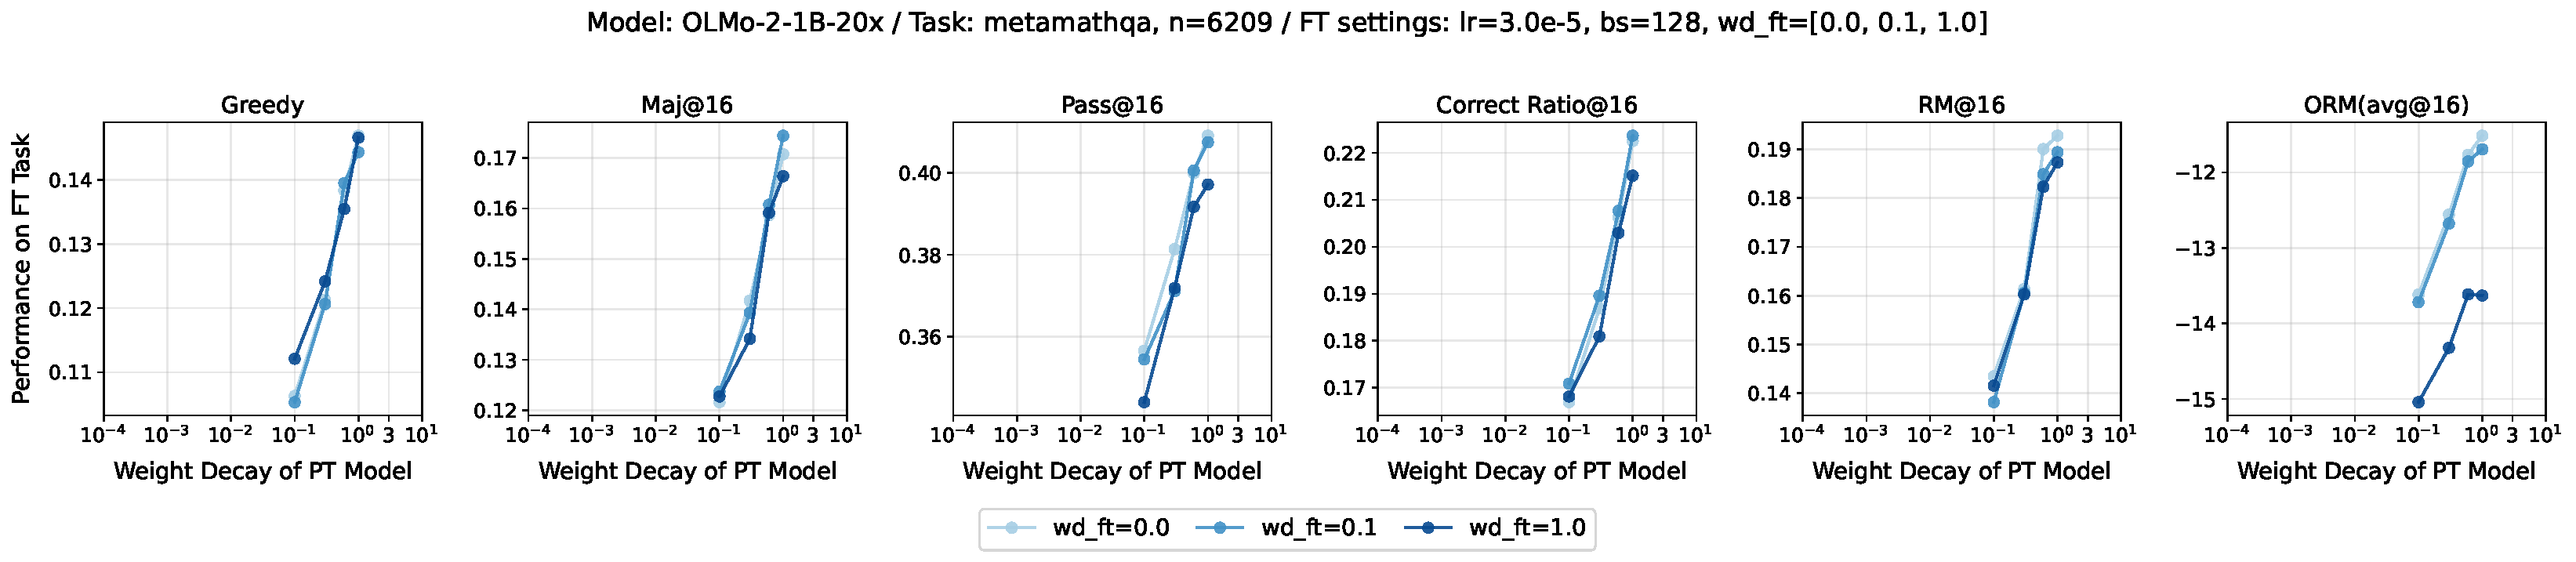
\includegraphics[width=0.92\textwidth, trim={0 25mm 0 25mm}, clip]{figs/a06_ft_sweep/ft_sweep_olmo-1B-30BT_metamathqa_lr3.0e-5_bs128.pdf}%
        }
    \end{subfigure}

    \begin{subfigure}[b]{\textwidth}
        \centering
        \makebox[\textwidth][c]{
            \hspace{-4mm}
            \raisebox{7.5mm}{\makebox[18mm][r]{\shortstack[l]{lr = 6e-5\\bs = 32}}}
            \hspace{2mm}
            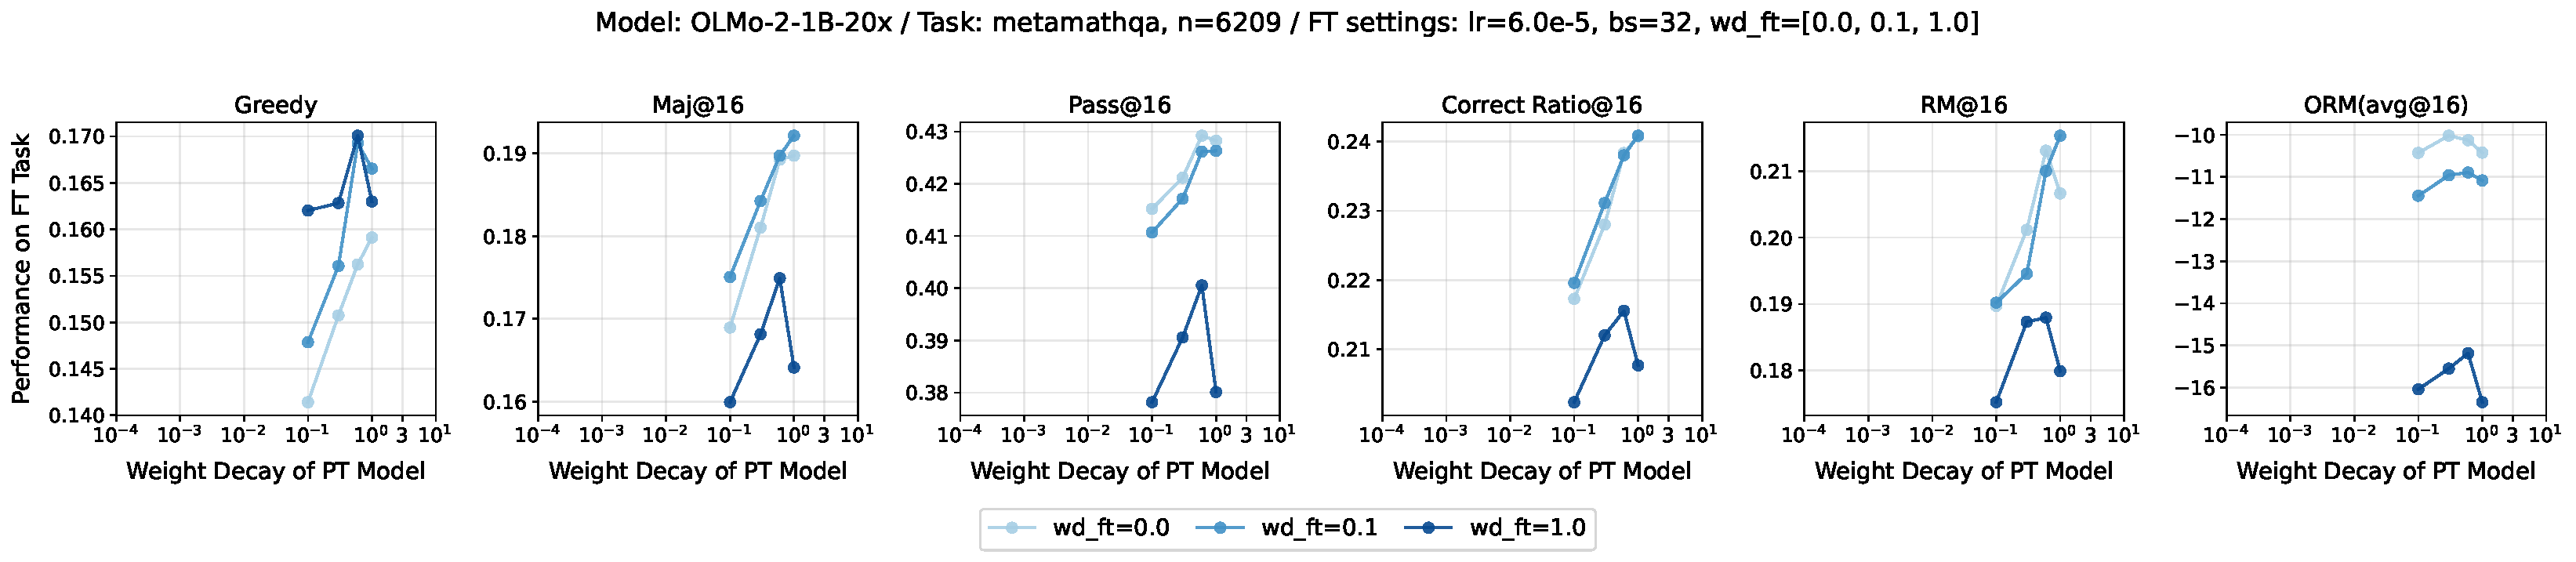
\includegraphics[width=0.92\textwidth, trim={0 25mm 0 25mm}, clip]{figs/a06_ft_sweep/ft_sweep_olmo-1B-30BT_metamathqa_lr6.0e-5_bs32.pdf}%
        }
    \end{subfigure}

    \begin{subfigure}[b]{\textwidth}
        \centering
        \makebox[\textwidth][c]{
            \hspace{-4mm}
            \raisebox{7.5mm}{\makebox[18mm][r]{\shortstack[l]{lr = 6e-5\\bs = 64}}}
            \hspace{2mm}
            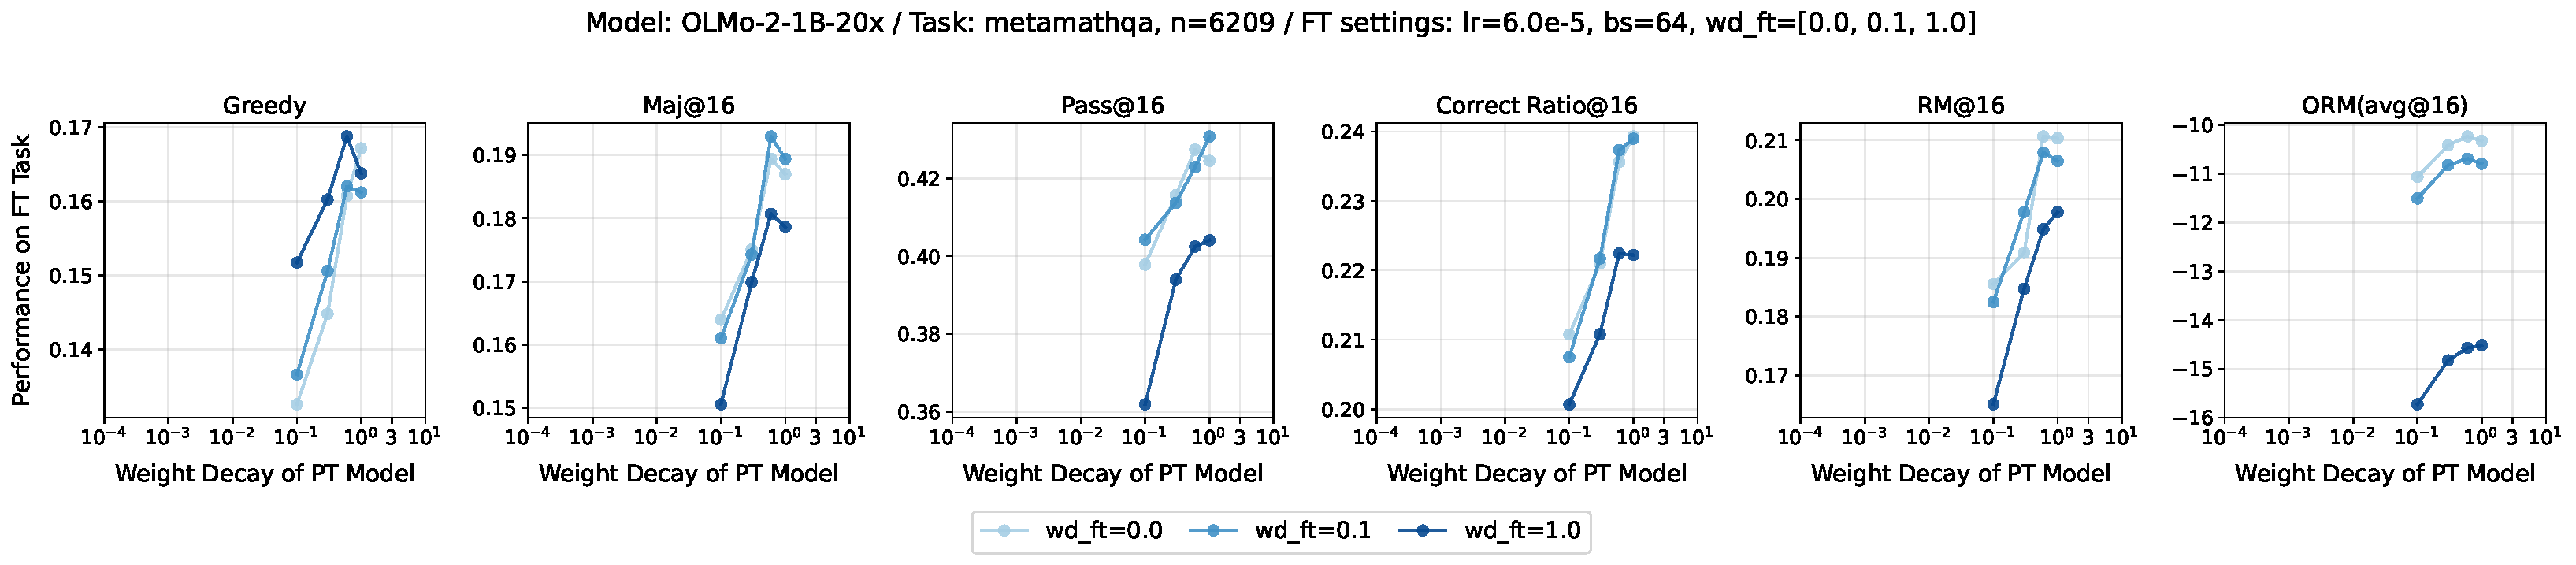
\includegraphics[width=0.92\textwidth, trim={0 25mm 0 25mm}, clip]{figs/a06_ft_sweep/ft_sweep_olmo-1B-30BT_metamathqa_lr6.0e-5_bs64.pdf}%
        }
    \end{subfigure}

    \begin{subfigure}[b]{\textwidth}
        \centering
        \makebox[\textwidth][c]{
            \hspace{-4mm}
            \raisebox{15mm}{\makebox[18mm][r]{\shortstack[l]{lr = 6e-5\\bs = 128}}}
            \hspace{2mm}
            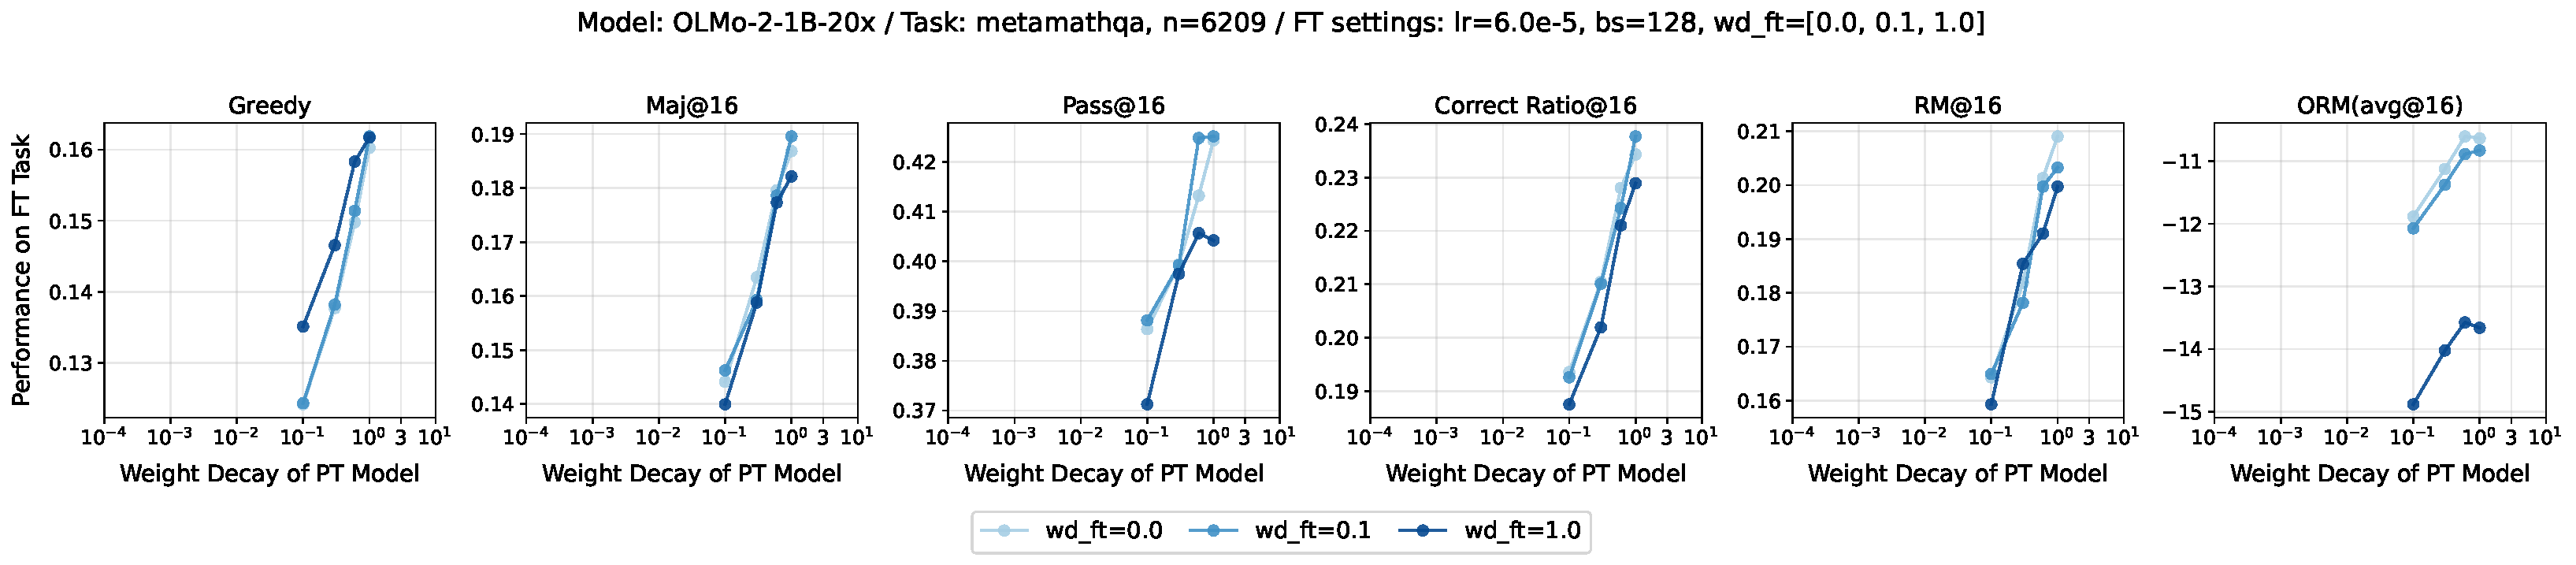
\includegraphics[width=0.92\textwidth, trim={0 0 0 25mm}, clip]{figs/a06_ft_sweep/ft_sweep_olmo-1B-30BT_metamathqa_lr6.0e-5_bs128.pdf}%
        }
    \end{subfigure}

    \caption{{\bf Effect of pretraining weight decay on fine-tuning performance for each set of fine-tuning hyperparameters: \metamathqa{}.} 
    \olmoonex{} models pretrained with different weight decay values (wd\_pt = [0.1, 0.3, 0.6, 1.0]) are fine-tuned on the \metamathqa{} dataset. We vary the learning rate (lr = [1e-5, 3e-5, 6e-5]), weight decay (wd\_ft = [0, 0.1, 1.0]), and batch size (bs = [32, 64, 128]) during fine-tuning.
    Average performance over all hyperparameters is shown in Figure~\ref{fig:app-ft-sweep--avg-and-max-perf}. Across fine-tuning hyperparameters and evaluation metrics, the higher the weight decay during pretraining, the better the downstream performance.}
    \label{fig:app-ft-sweep--metamathqa}
\end{figure*}



\begin{figure*}[h] 
    \centering

    \begin{subfigure}[b]{\textwidth}
        \centering
        \makebox[\textwidth][c]{%
            \hspace{-4mm}%
            \raisebox{7.5mm}{\makebox[18mm][r]{\shortstack[l]{lr = 1e-5\\bs = 32}}}%
            \hspace{2mm}%
            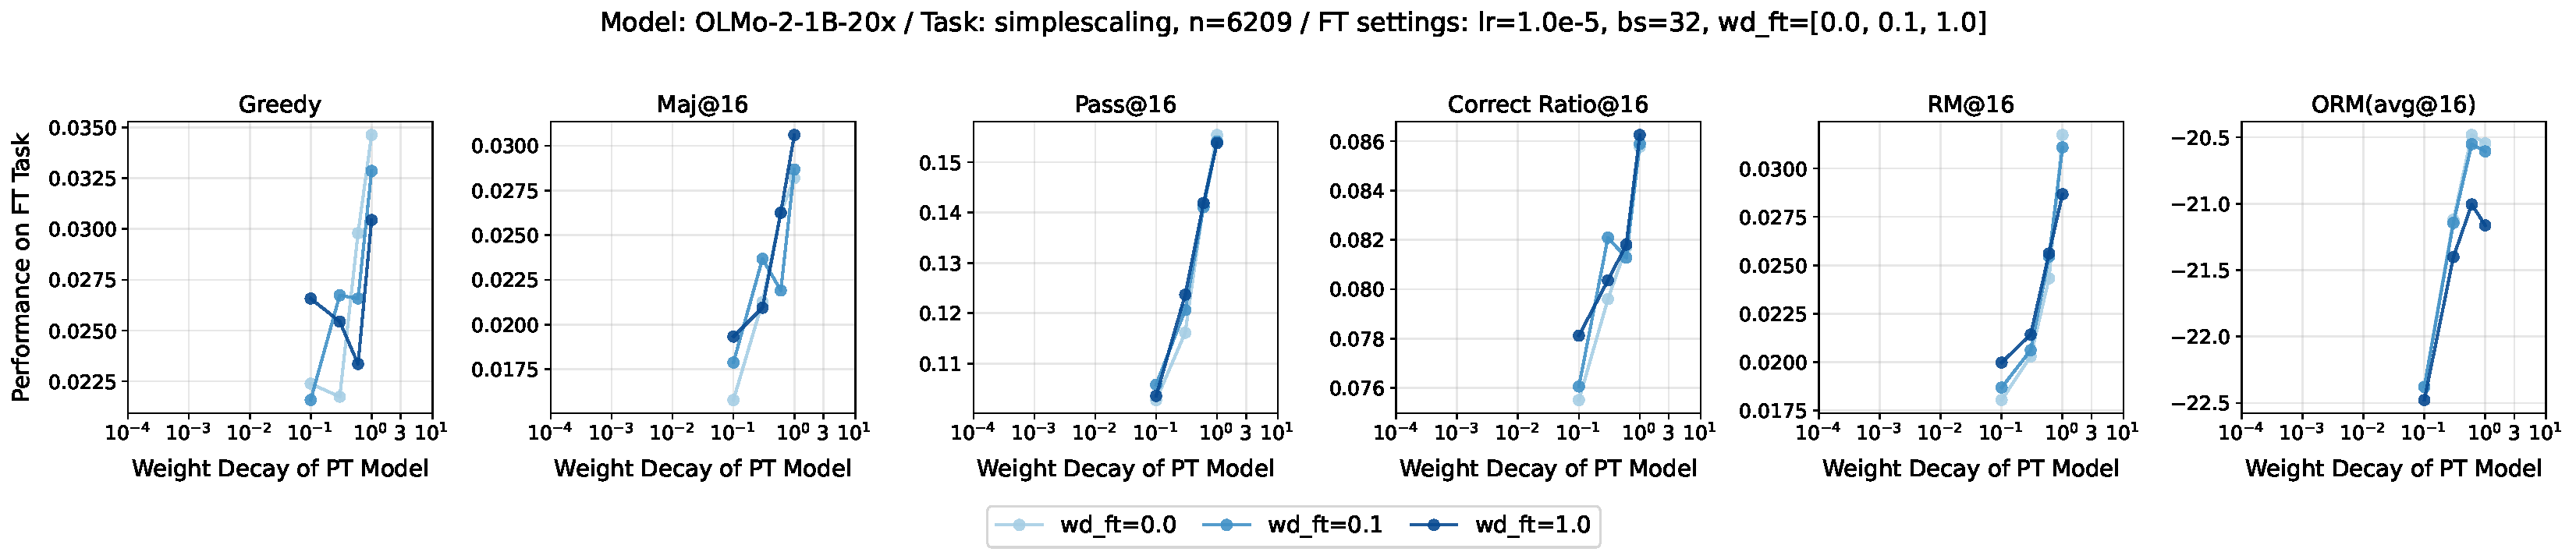
\includegraphics[width=0.92\textwidth, trim={0 25mm 0 20mm}, clip]{figs/a06_ft_sweep/ft_sweep_olmo-1B-30BT_simplescaling_lr1.0e-5_bs32.pdf}%
        }
    \end{subfigure}

    \begin{subfigure}[b]{\textwidth}
        \centering
        \makebox[\textwidth][c]{%
            \hspace{-4mm}%
            \raisebox{7.5mm}{\makebox[18mm][r]{\shortstack[l]{lr = 1e-5\\bs = 64}}}%
            \hspace{2mm}%
            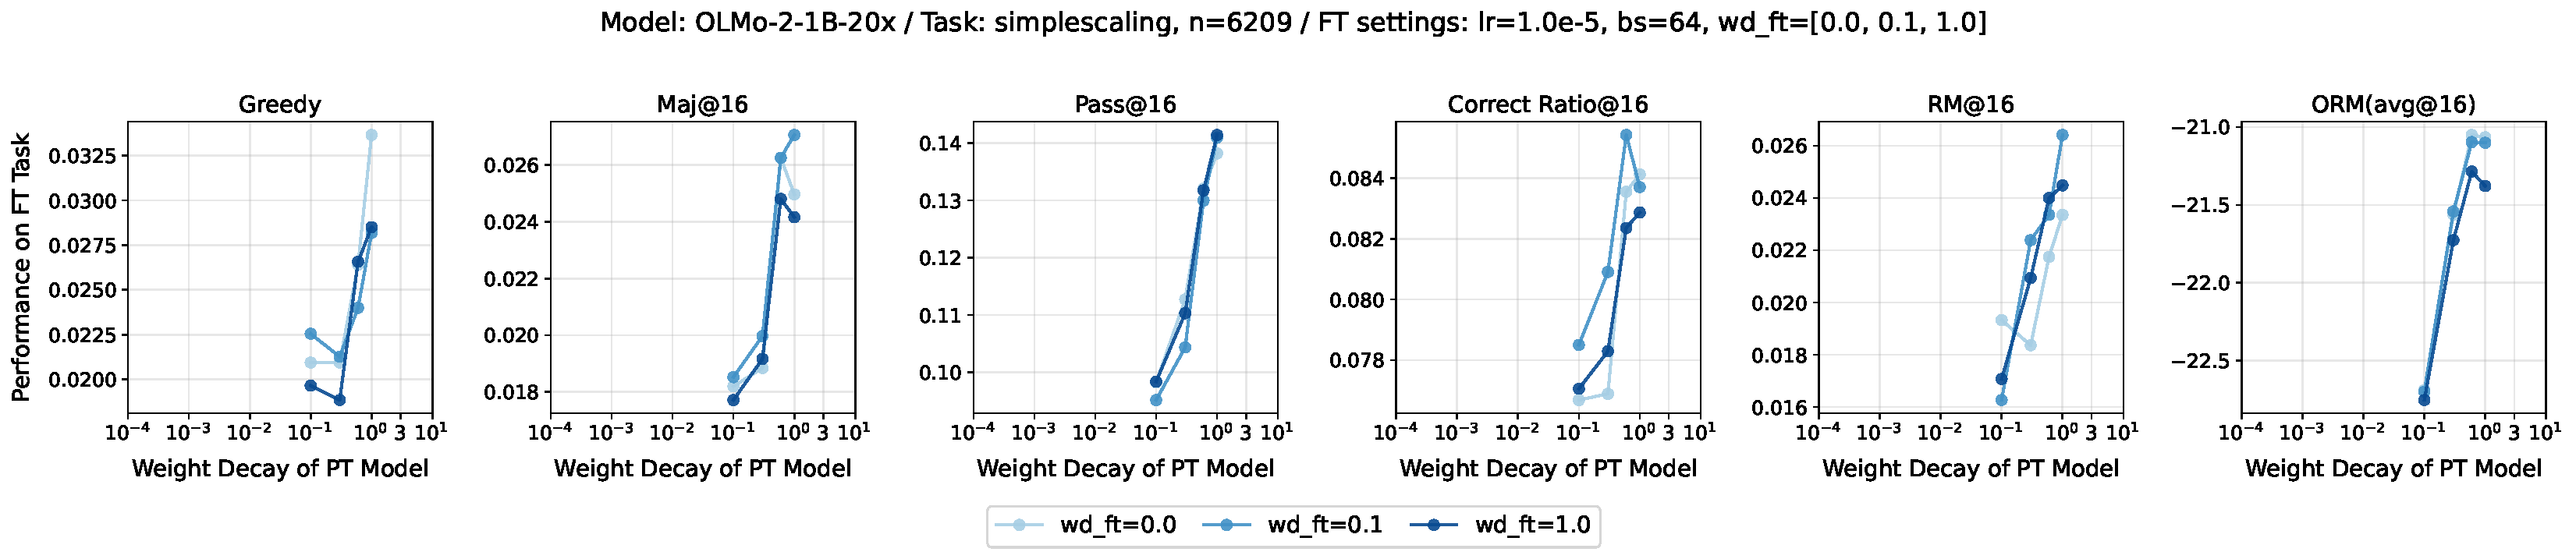
\includegraphics[width=0.92\textwidth, trim={0 25mm 0 25mm}, clip]{figs/a06_ft_sweep/ft_sweep_olmo-1B-30BT_simplescaling_lr1.0e-5_bs64.pdf}%
        }
    \end{subfigure}

    \begin{subfigure}[b]{\textwidth}
        \centering
        \makebox[\textwidth][c]{%
            \hspace{-4mm}%
            \raisebox{7.5mm}{\makebox[18mm][r]{\shortstack[l]{lr = 1e-5\\bs = 128}}}%
            \hspace{2mm}%
            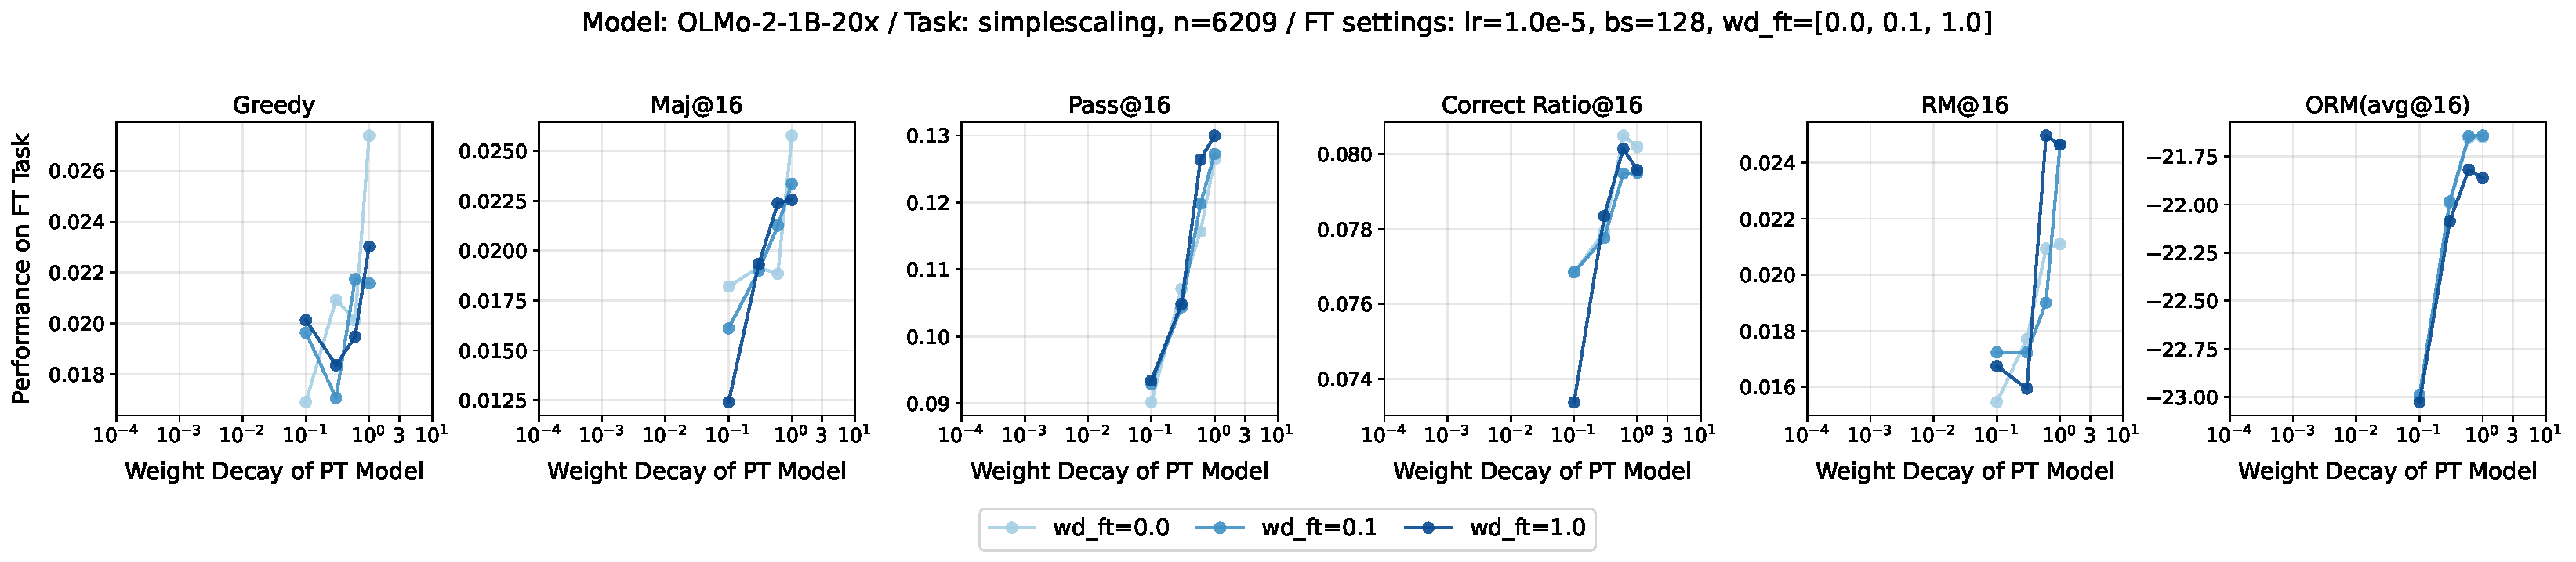
\includegraphics[width=0.92\textwidth, trim={0 25mm 0 25mm}, clip]{figs/a06_ft_sweep/ft_sweep_olmo-1B-30BT_simplescaling_lr1.0e-5_bs128.pdf}%
        }
    \end{subfigure}

    \begin{subfigure}[b]{\textwidth}
        \centering
        \makebox[\textwidth][c]{%
            \hspace{-4mm}%
            \raisebox{7.5mm}{\makebox[18mm][r]{\shortstack[l]{lr = 3e-5\\bs = 32}}}%
            \hspace{2mm}%
            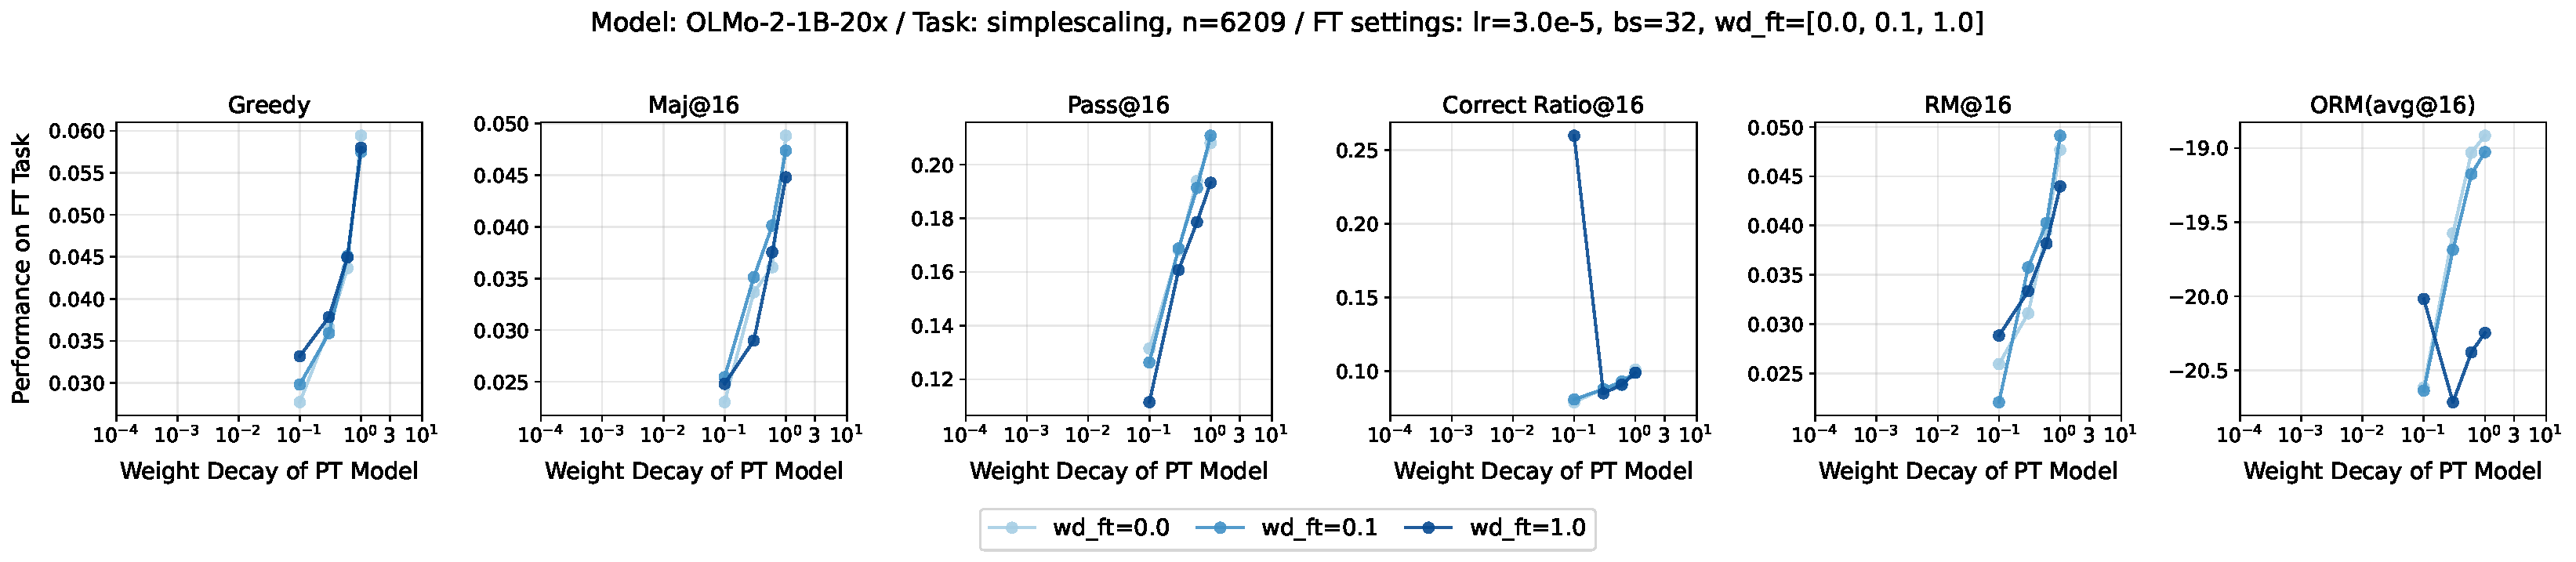
\includegraphics[width=0.92\textwidth, trim={0 25mm 0 25mm}, clip]{figs/a06_ft_sweep/ft_sweep_olmo-1B-30BT_simplescaling_lr3.0e-5_bs32.pdf}%
        }
    \end{subfigure}

    \begin{subfigure}[b]{\textwidth}
        \centering
        \makebox[\textwidth][c]{%
            \hspace{-4mm}%
            \raisebox{7.5mm}{\makebox[18mm][r]{\shortstack[l]{lr = 3e-5\\bs = 64}}}%
            \hspace{2mm}%
            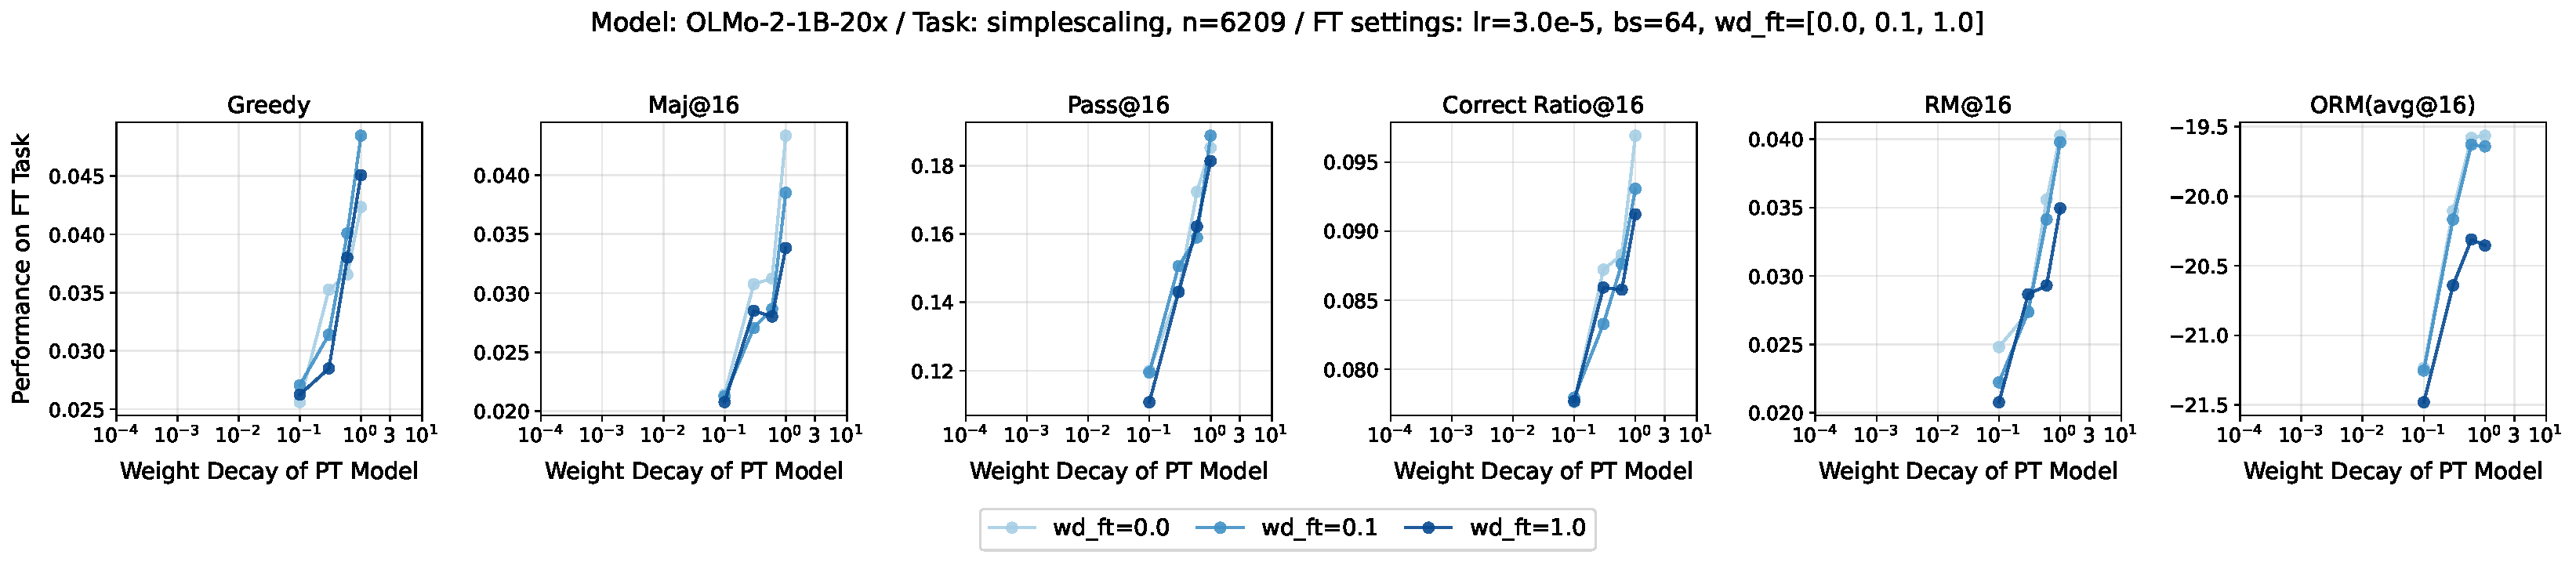
\includegraphics[width=0.92\textwidth, trim={0 25mm 0 25mm}, clip]{figs/a06_ft_sweep/ft_sweep_olmo-1B-30BT_simplescaling_lr3.0e-5_bs64.pdf}%
        }
    \end{subfigure}

    \begin{subfigure}[b]{\textwidth}
        \centering
        \makebox[\textwidth][c]{%
            \hspace{-4mm}%
            \raisebox{7.5mm}{\makebox[18mm][r]{\shortstack[l]{lr = 3e-5\\bs = 128}}}%
            \hspace{2mm}%
            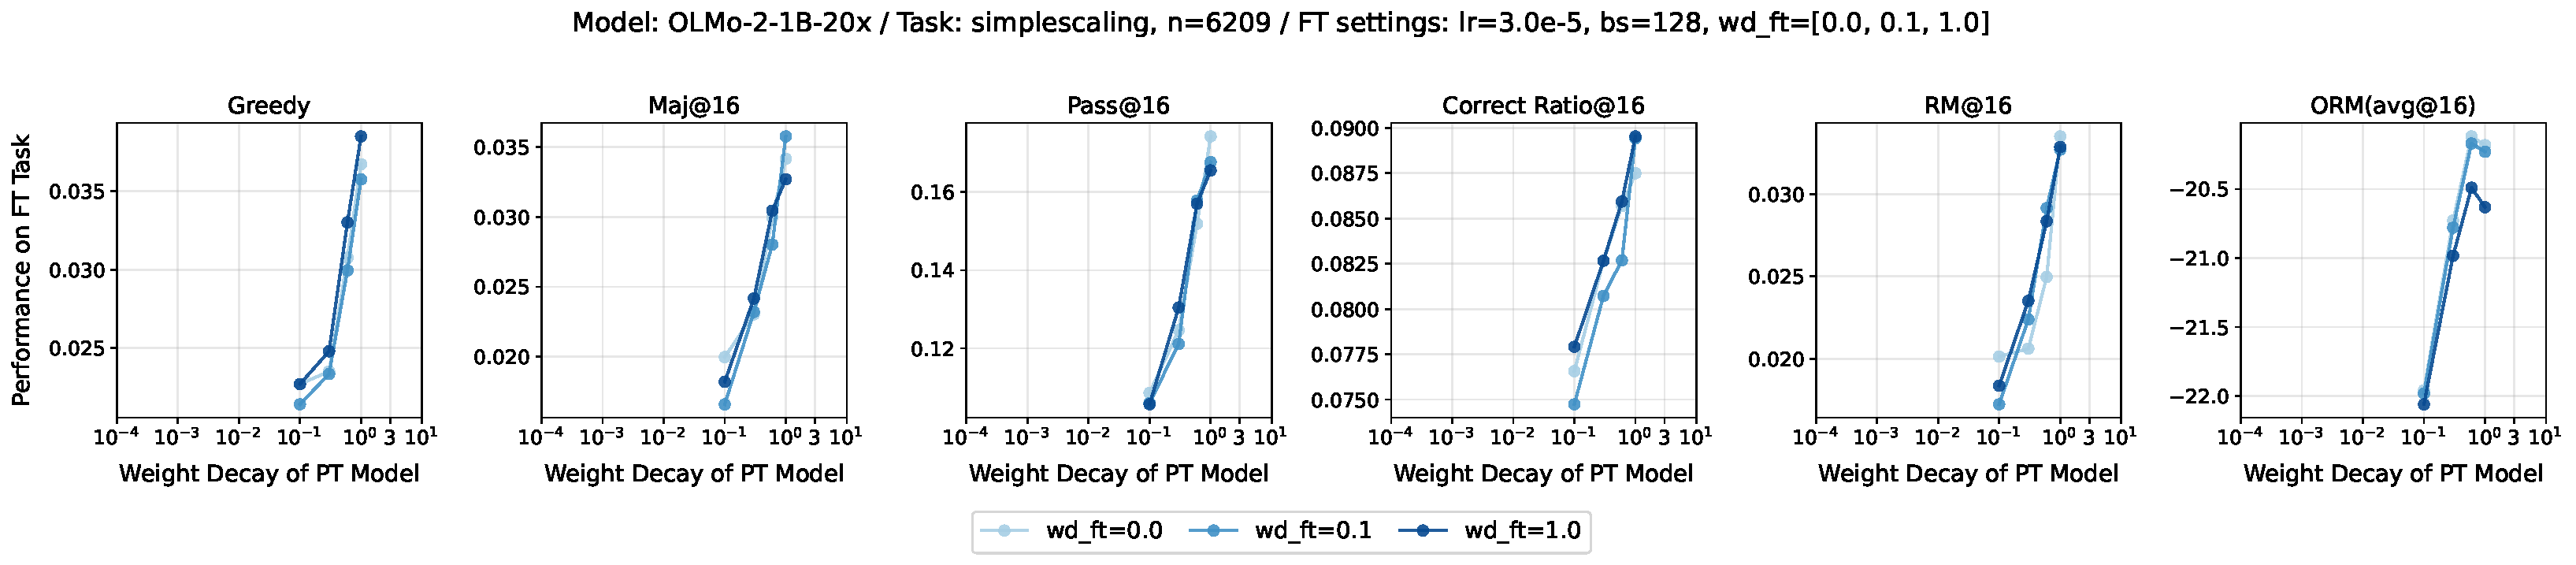
\includegraphics[width=0.92\textwidth, trim={0 25mm 0 25mm}, clip]{figs/a06_ft_sweep/ft_sweep_olmo-1B-30BT_simplescaling_lr3.0e-5_bs128.pdf}%
        }
    \end{subfigure}

    \begin{subfigure}[b]{\textwidth}
        \centering
        \makebox[\textwidth][c]{%
            \hspace{-4mm}%
            \raisebox{7.5mm}{\makebox[18mm][r]{\shortstack[l]{lr = 6e-5\\bs = 32}}}%
            \hspace{2mm}%
            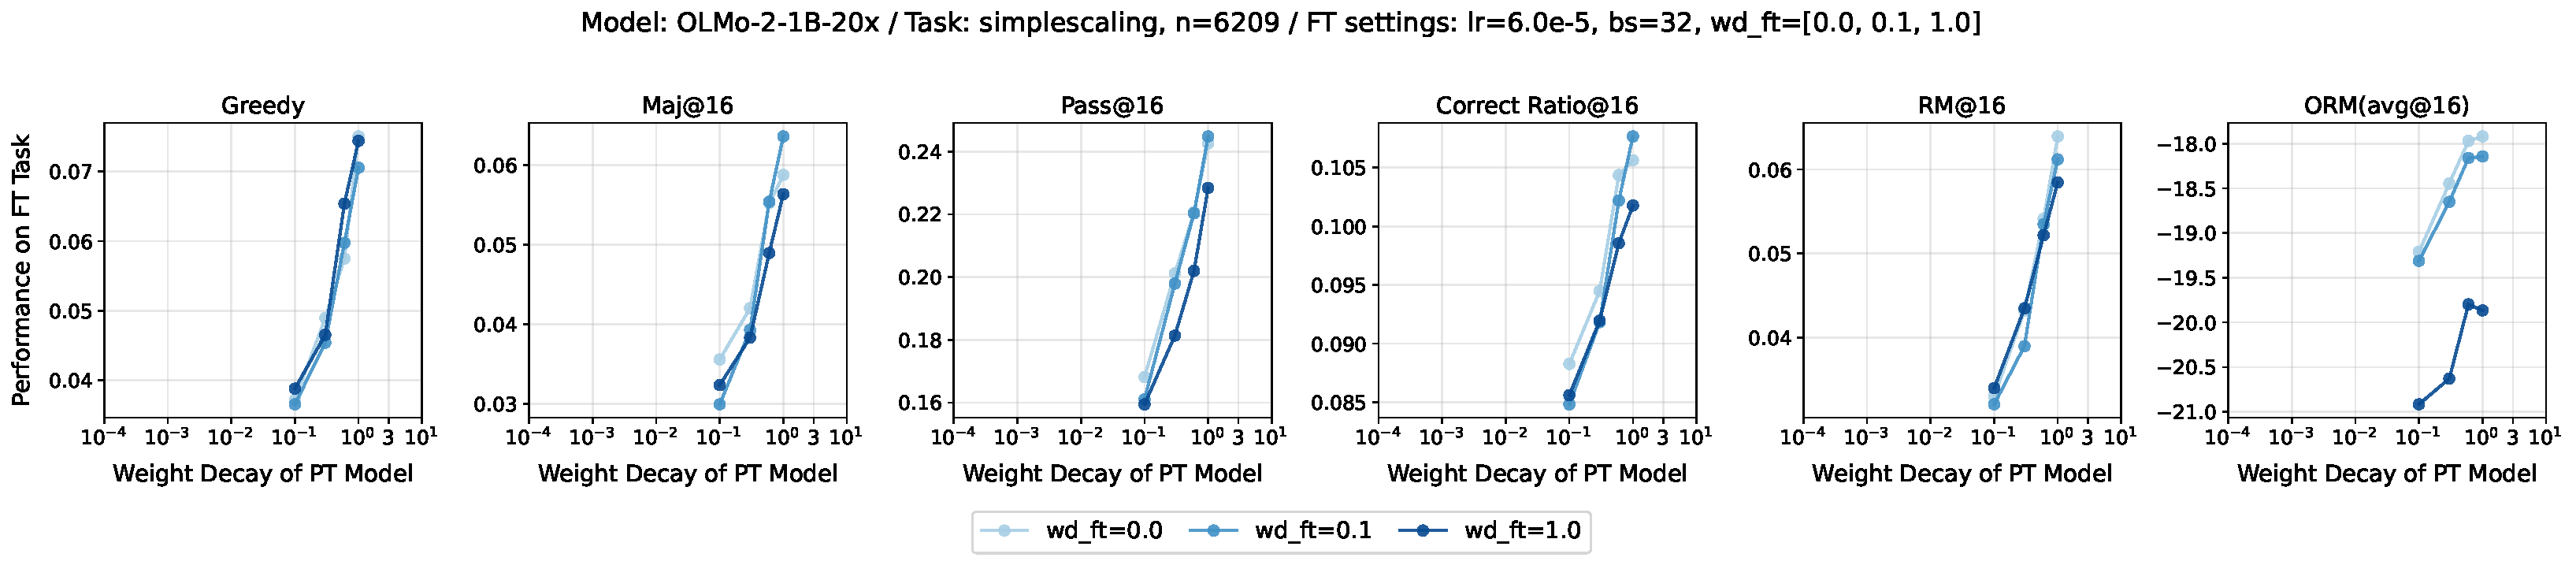
\includegraphics[width=0.92\textwidth, trim={0 25mm 0 25mm}, clip]{figs/a06_ft_sweep/ft_sweep_olmo-1B-30BT_simplescaling_lr6.0e-5_bs32.pdf}%
        }
    \end{subfigure}

    \begin{subfigure}[b]{\textwidth}
        \centering
        \makebox[\textwidth][c]{%
            \hspace{-4mm}%
            \raisebox{7.5mm}{\makebox[18mm][r]{\shortstack[l]{lr = 6e-5\\bs = 64}}}%
            \hspace{2mm}%
            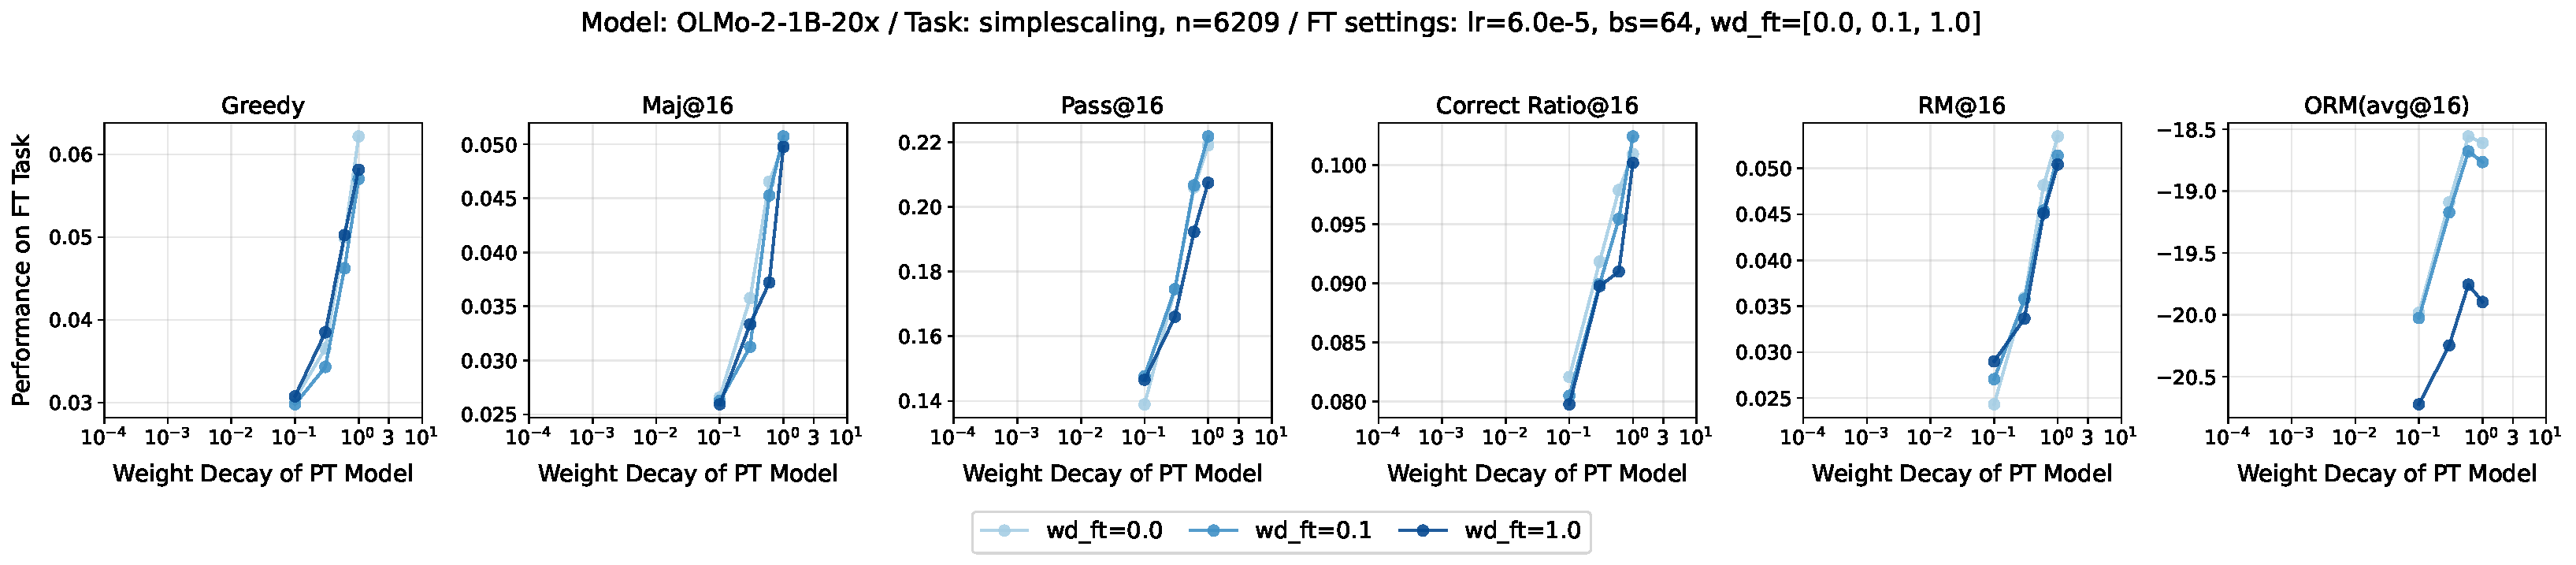
\includegraphics[width=0.92\textwidth, trim={0 25mm 0 25mm}, clip]{figs/a06_ft_sweep/ft_sweep_olmo-1B-30BT_simplescaling_lr6.0e-5_bs64.pdf}%
        }
    \end{subfigure}

    \begin{subfigure}[b]{\textwidth}
        \centering
        \makebox[\textwidth][c]{%
            \hspace{-4mm}%
            \raisebox{15mm}{\makebox[18mm][r]{\shortstack[l]{lr = 6e-5\\bs = 128}}}%
            \hspace{2mm}%
            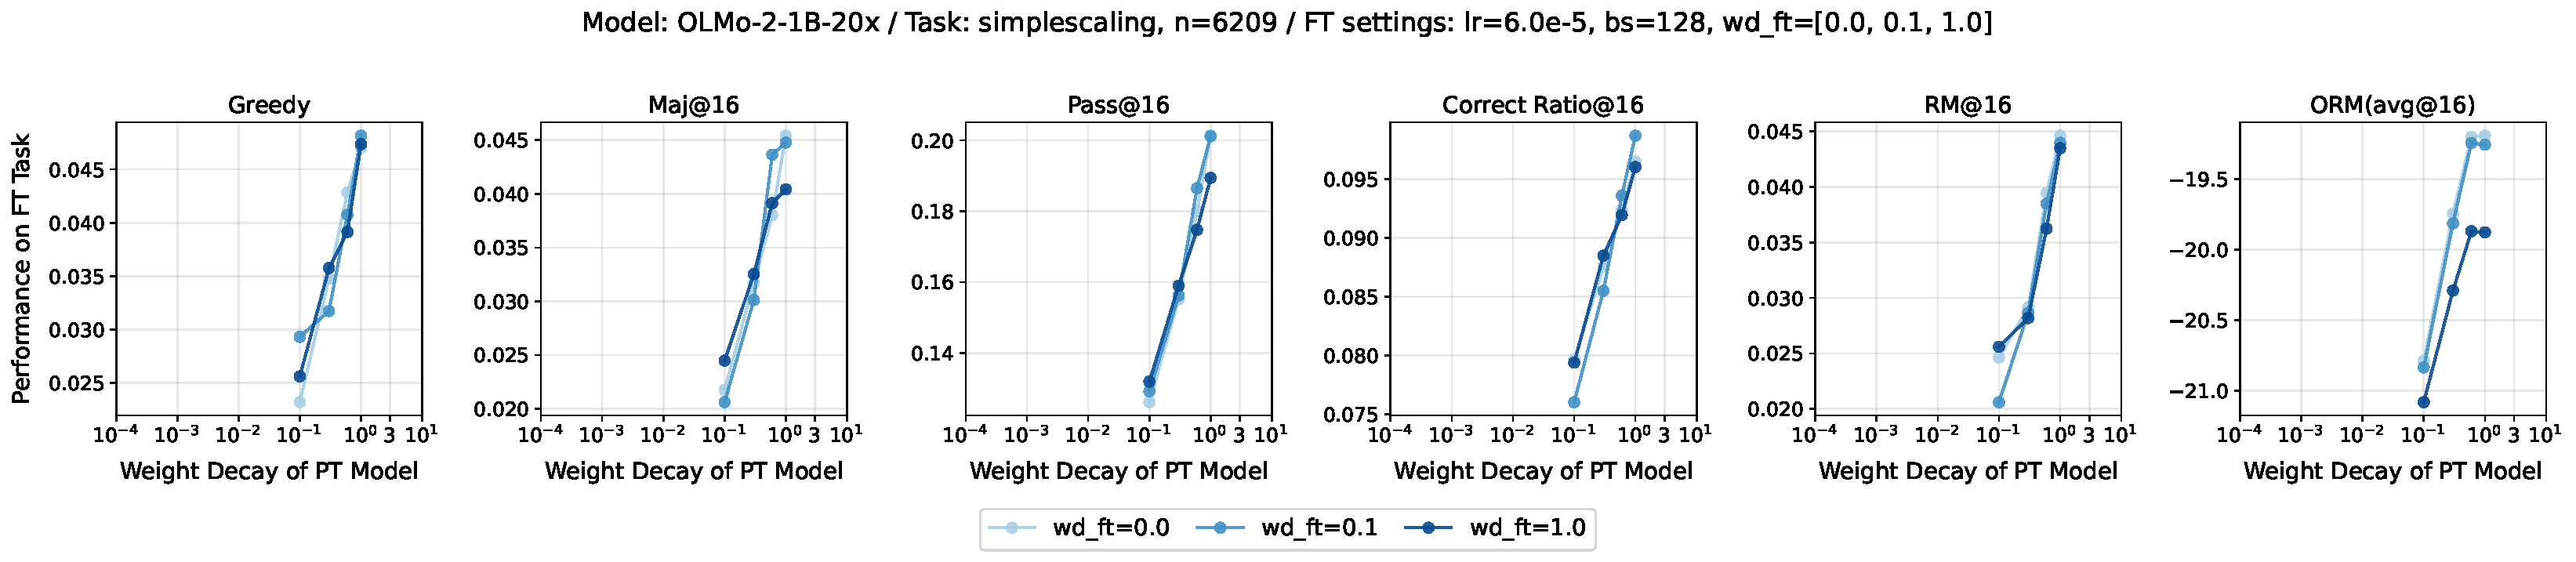
\includegraphics[width=0.92\textwidth, trim={0 0 0 25mm}, clip]{figs/a06_ft_sweep/ft_sweep_olmo-1B-30BT_simplescaling_lr6.0e-5_bs128.pdf}%
        }
    \end{subfigure}

    \caption{{\bf Effect of pretraining weight decay on fine-tuning performance for each set of fine-tuning hyperparameters: \simplescaling{}.} 
    \olmoonex{} models pretrained with different weight decay values (wd\_pt = [0.1, 0.3, 0.6, 1.0]) are fine-tuned on the \simplescaling{} dataset. We vary the learning rate (lr = [1e-5, 3e-5, 6e-5]), weight decay (wd\_ft = [0, 0.1, 1.0]), and batch size (bs = [32, 64, 128]) during fine-tuning.
    Average performance over all hyperparameters is shown in Figure~\ref{fig:app-ft-sweep--avg-and-max-perf}. Across fine-tuning hyperparameters and evaluation metrics, the higher the weight decay during pretraining, the better the downstream performance.}
    \label{fig:app-ft-sweep--simplescaling}
\end{figure*}







\begin{figure*}[h] 
    \centering

    \begin{subfigure}[b]{\textwidth}
        \centering
        \makebox[\textwidth][c]{%
            \hspace{-4mm}%
            \raisebox{7.5mm}{\makebox[18mm][r]{\shortstack[l]{\metamathqa{},\\Average}}}%
            \hspace{2mm}%
            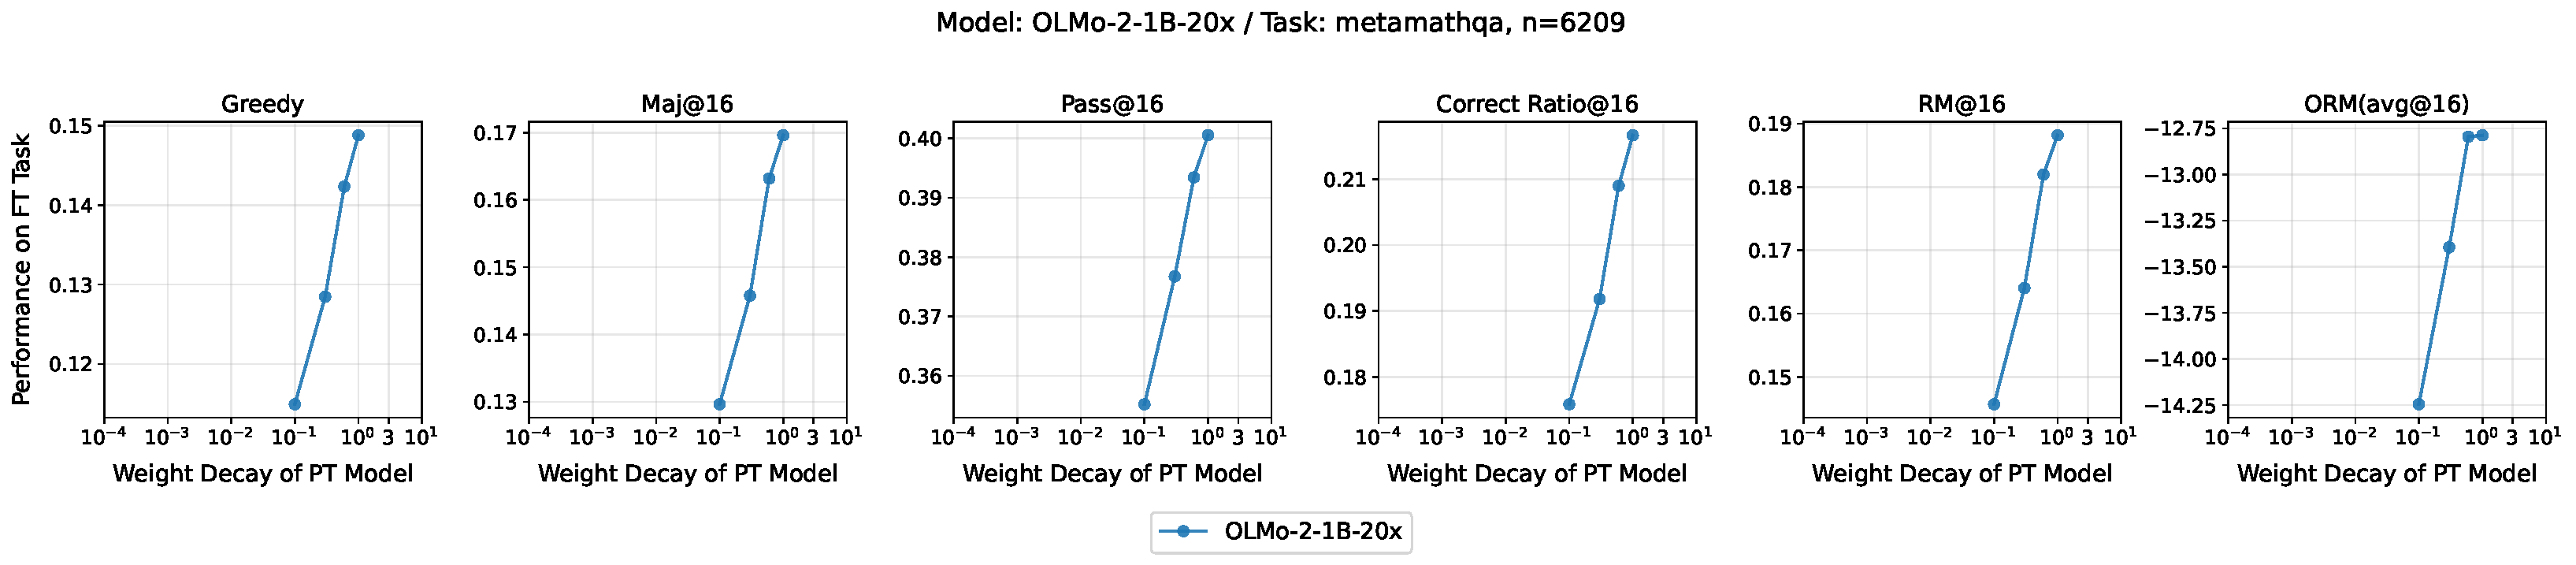
\includegraphics[width=0.92\textwidth, trim={0 25mm 0 20mm}, clip]{figs/a06_ft_sweep/ft_sweep_olmo-1B-30BT_metamathqa_average.pdf}%
        }
    \end{subfigure}

    \begin{subfigure}[b]{\textwidth}
        \centering
        \makebox[\textwidth][c]{%
            \hspace{-4mm}%
            \raisebox{7.5mm}{\makebox[18mm][r]{\shortstack[l]{\metamathqa{},\\Maximum}}}%
            \hspace{2mm}%
            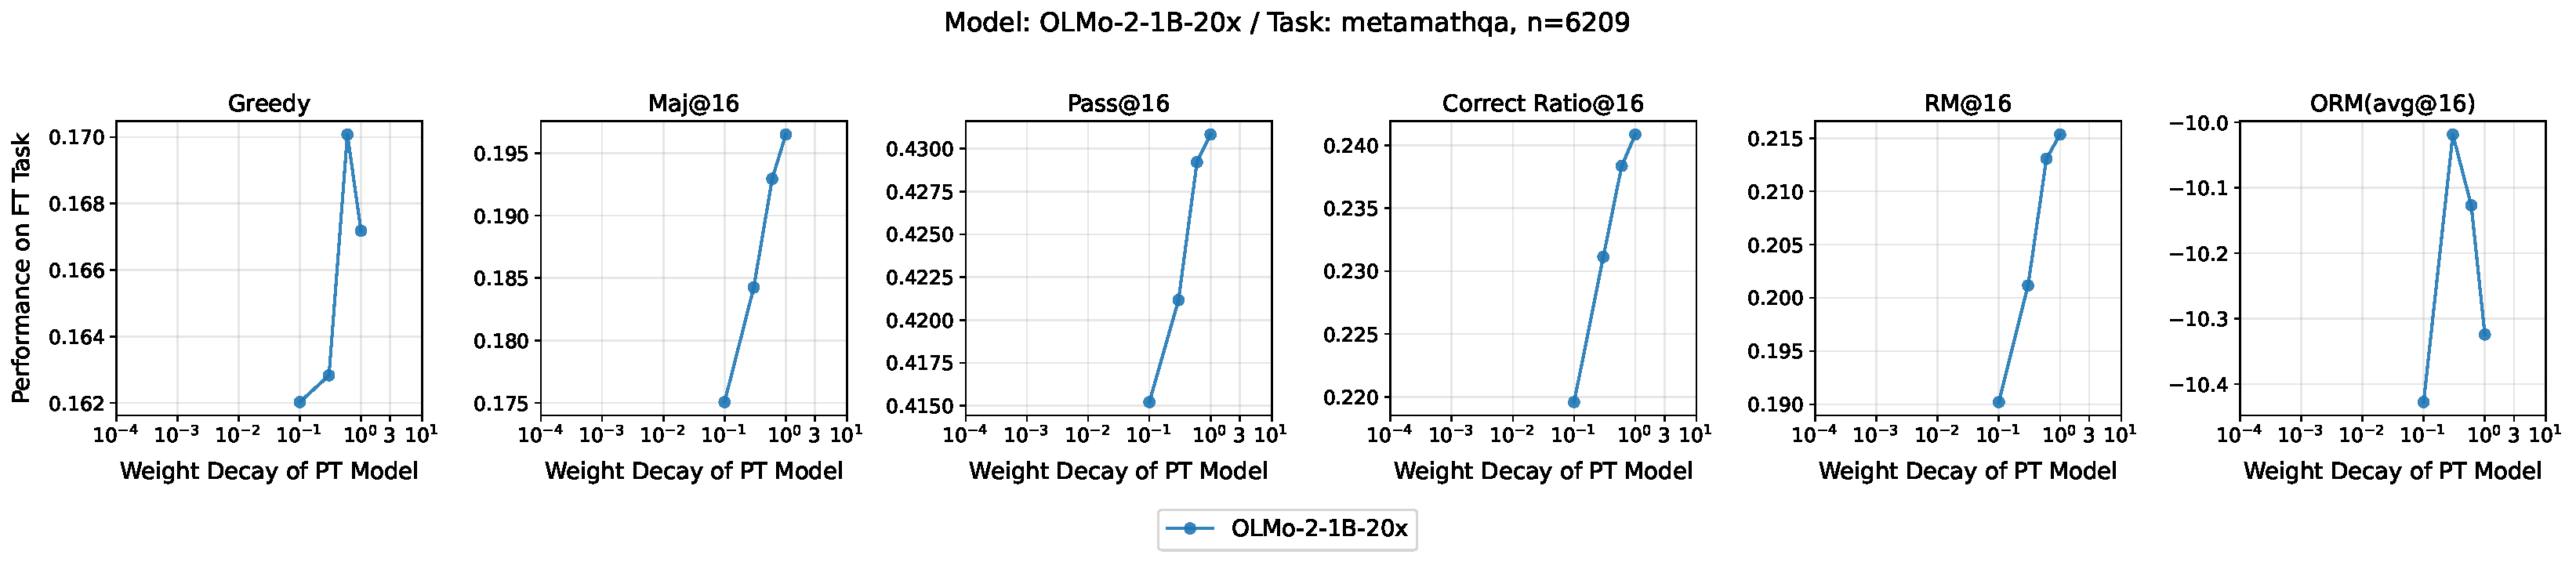
\includegraphics[width=0.92\textwidth, trim={0 25mm 0 25mm}, clip]{figs/a06_ft_sweep/ft_sweep_olmo-1B-30BT_metamathqa_max.pdf}%
        }
    \end{subfigure}

    \begin{subfigure}[b]{\textwidth}
        \centering
        \makebox[\textwidth][c]{%
            \hspace{-4mm}%
            \raisebox{7.5mm}{\makebox[18mm][r]{\shortstack[l]{\simplescaling{},\\Average}}}%
            \hspace{2mm}%
            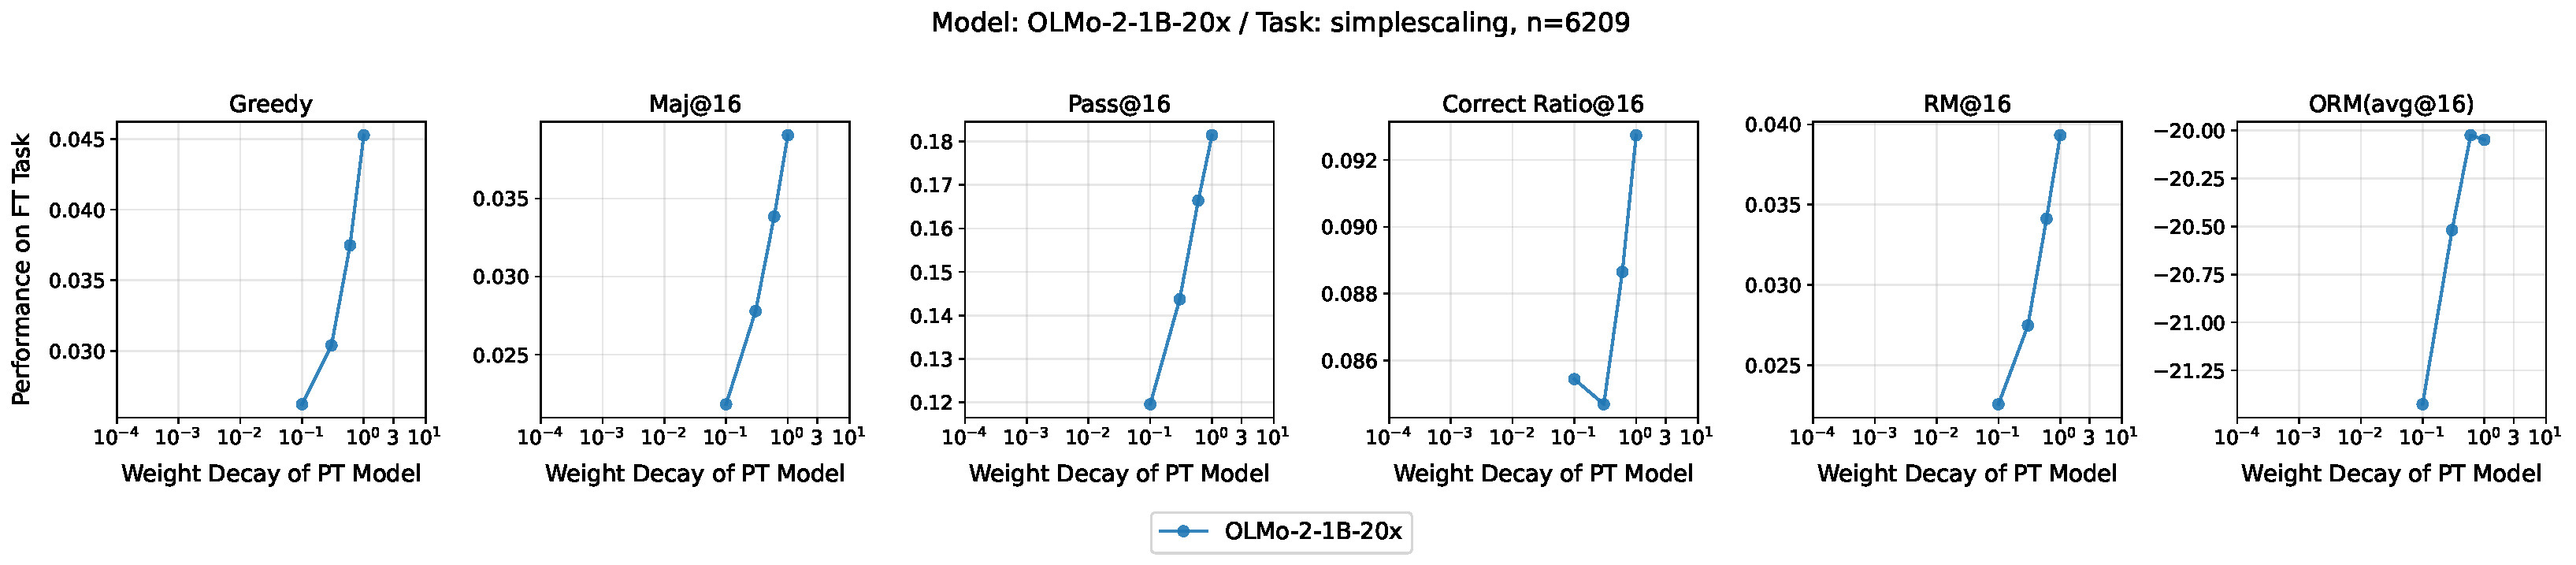
\includegraphics[width=0.92\textwidth, trim={0 25mm 0 25mm}, clip]{figs/a06_ft_sweep/ft_sweep_olmo-1B-30BT_simplescaling_average.pdf}%
        }
    \end{subfigure}

    \begin{subfigure}[b]{\textwidth}
        \centering
        \makebox[\textwidth][c]{%
            \hspace{-4mm}%
            \raisebox{7.5mm}{\makebox[18mm][r]{\shortstack[l]{\simplescaling{},\\Maximum}}}%
            \hspace{2mm}%
            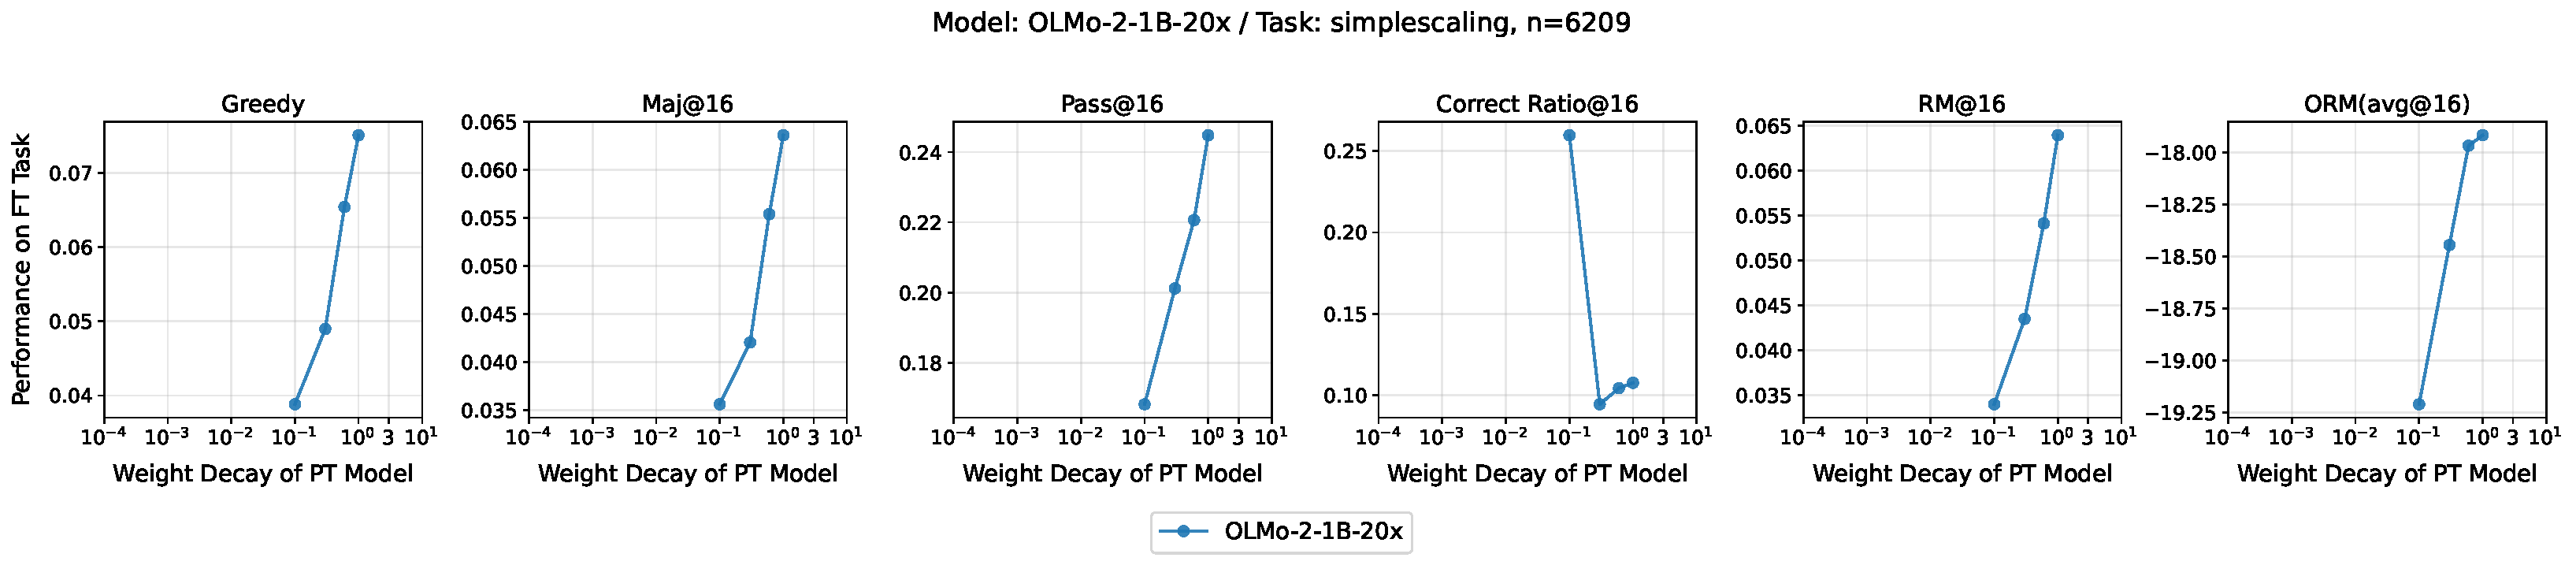
\includegraphics[width=0.92\textwidth, trim={0 25mm 0 25mm}, clip]{figs/a06_ft_sweep/ft_sweep_olmo-1B-30BT_simplescaling_max.pdf}%
        }
    \end{subfigure}

    \begin{subfigure}[b]{\textwidth}
        \centering
        \makebox[\textwidth][c]{%
            \hspace{-4mm}%
            \raisebox{7.5mm}{\makebox[18mm][r]{\shortstack[l]{Both datasets,\\Average}}}%
            \hspace{2mm}%
            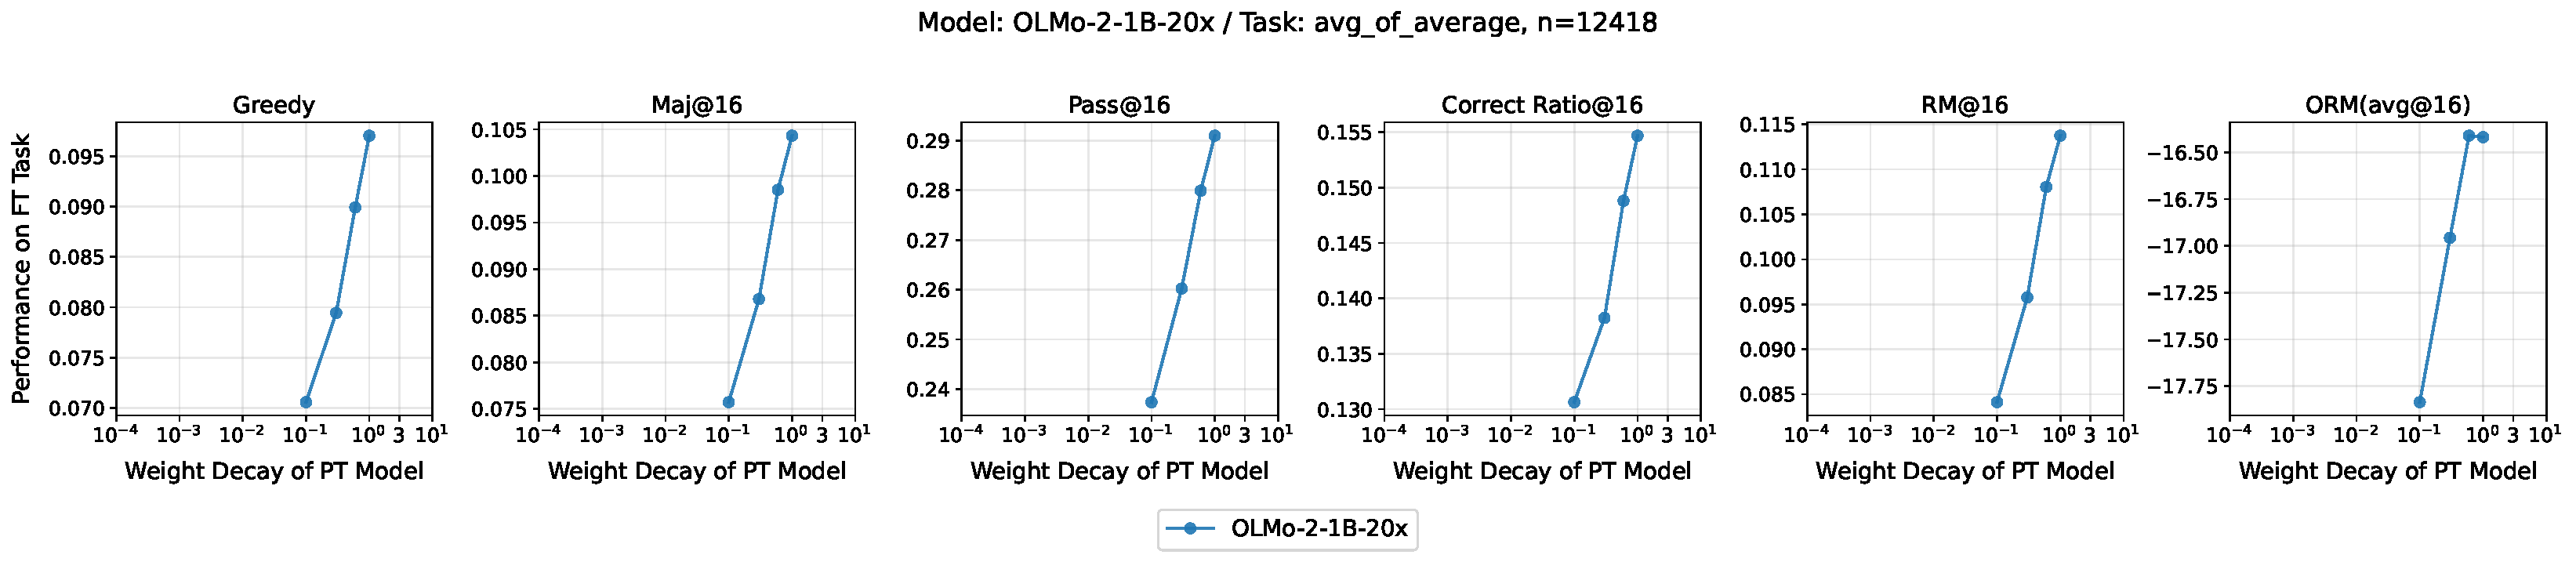
\includegraphics[width=0.92\textwidth, trim={0 25mm 0 25mm}, clip]{figs/a06_ft_sweep/ft_sweep_olmo-1B-30BT_avg_of_average_average.pdf}%
        }
    \end{subfigure}

    \begin{subfigure}[b]{\textwidth}
        \centering
        \makebox[\textwidth][c]{%
            \hspace{-4mm}%
            \raisebox{7.5mm}{\makebox[18mm][r]{\shortstack[l]{Both datasets,\\Maximum}}}%
            \hspace{2mm}%
            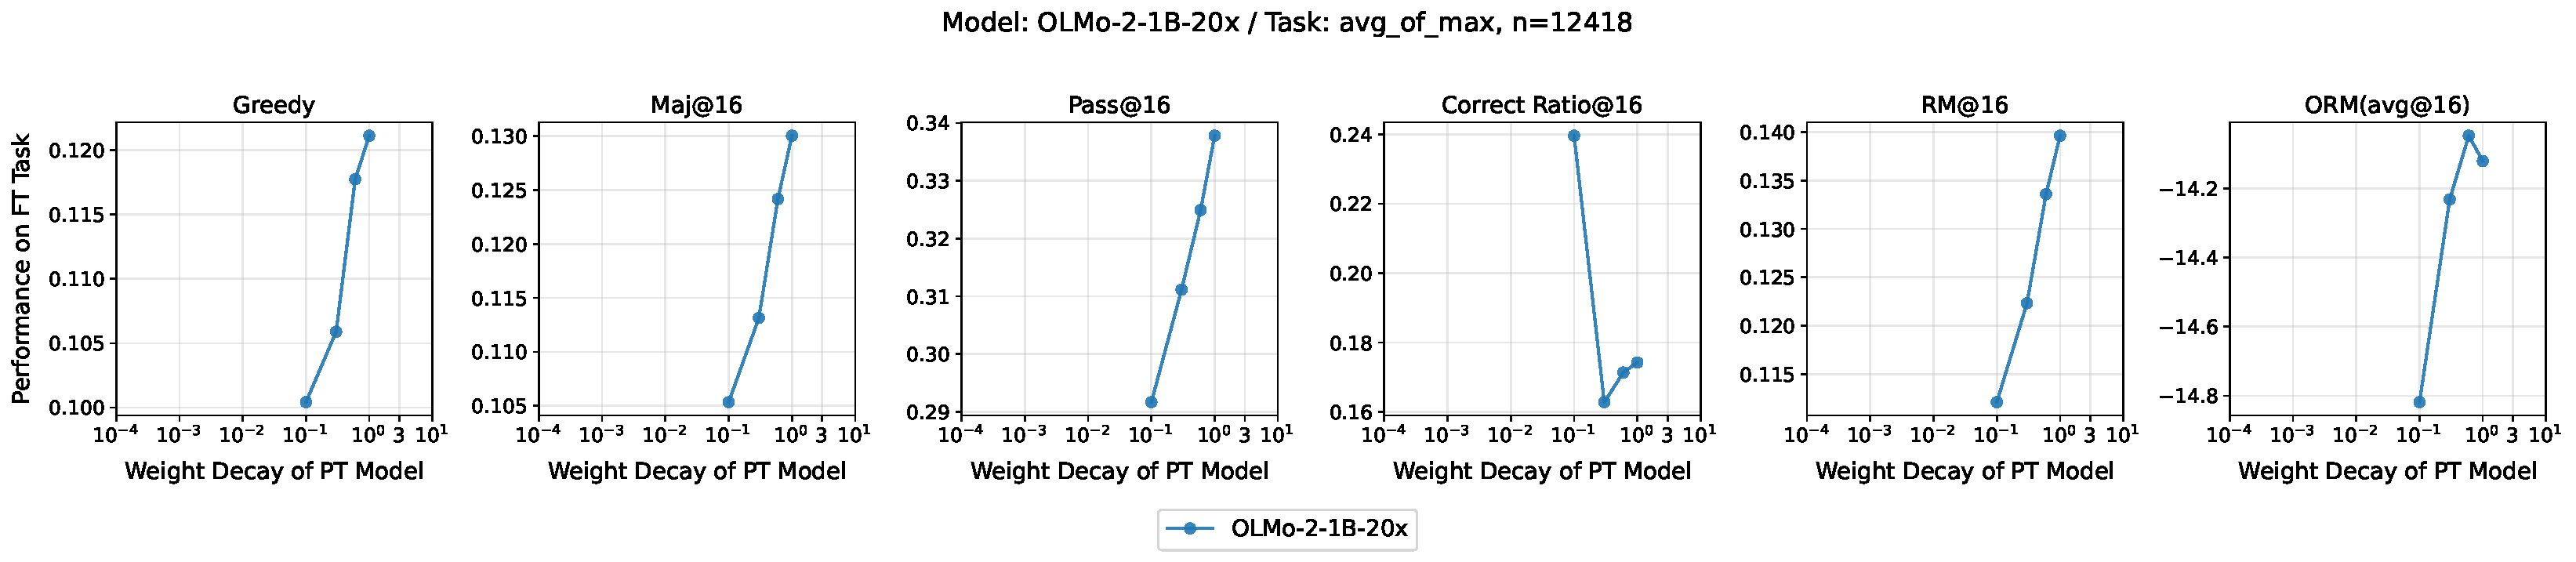
\includegraphics[width=0.92\textwidth, trim={0 25mm 0 25mm}, clip]{figs/a06_ft_sweep/ft_sweep_olmo-1B-30BT_avg_of_max_max.pdf}%
        }
    \end{subfigure}

    \caption{{\bf Effect of pretraining weight decay on fine-tuning performance for the average and best set of fine-tuning hyperparameters.} 
    This figure shows the average fine-tuning performance (Rows 1, 3, 5) and the best fine-tuning performance (Rows 2, 4, 6) over all the fine-tuning hyperparameter combinations. The higher the weight decay during pretraining, the better the fine-tuning performance.}
    \label{fig:app-ft-sweep--avg-and-max-perf}
\end{figure*}

